% This is samplepaper.tex, a sample chapter demonstrating the
% LLNCS macro package for Springer Computer Science proceedings;
% Version 2.20 of 2017/10/04
%
\documentclass[runningheads]{llncs}
\usepackage{amsmath}
\usepackage{amssymb}
\usepackage{mathrsfs}
\usepackage{graphicx}
\usepackage{subfigure}
\usepackage{physics}
\usepackage{tikz} 
\usepackage{scalefnt}
\usepackage{qcircuit}
\usepackage{tabularx} 
\usepackage{float}
\usepackage{multirow}

\usepackage[linesnumbered,ruled,lined]{algorithm2e}
% Used for displaying a sample figure. If possible, figure files should
% be included in EPS format.
%
% If you use the hyperref package, please uncomment the following line
% to display URLs in blue roman font according to Springer's eBook style:
% \renewcommand\UrlFont{\color{blue}\rmfamily}

\begin{document}
%
\title{Quantum Circuit Transformation Based on Subgraph Isomorphism and Tabu Search\thanks{Supported by organization x.}}
%
%\titlerunning{Abbreviated paper title}
% If the paper title is too long for the running head, you can set
% an abbreviated paper title here
%
\author{First Aaaaaaauthor\inst{1}\orcidID{0000-ereer1111-2222-3333} \and
Second Author\inst{2,3}\orcidID{1111-2222-3333-4444} \and
Third Author\inst{3}\orcidID{2222--3333-4444-5555}}
%
\authorrunning{F. Author et al.}
% First names are abbreviated in the running head.
% If there are more than two authors, 'et al.' is used.
%
\institute{Princeton University, Princeton NJ 08544, USA \and
Springer Heidelberg, Tiergartenstr. 17, 69121 Heidelberg, Germany
\email{lncs@springer.com}\\
\url{http://www.springer.com/gp/computer-science/lncs} \and
ABC Institute, Rupert-Karls-University Heidelberg, Heidelberg, Germany\\
\email{\{abc,lncs\}@uni-heidelberg.de}}
%
\maketitle              % typeset the header of the contribution
%
\begin{abstract}
	The process of circuit transformation is to find an automatic method to map any logical quantum circuits to physical circuits effectively in an acceptable time, and add as few auxiliary gates as possible. We mainly propose an initial mapping algorithm based on a combined subgraph isomorphism algorithm and a circuit transformation algorithm based on Tabu Search ($QCTS$). Our experimental results show that the algorithm is effective. Compared with the initial mapping based on the $VF2$ algorithm, auxiliary gates added to our initial mapping are reduced by 22.26\%, and the depth of the output circuit is reduced by 11.17\%. $QCTS$ is scalable on large-scale circuits with less overhead, compared with other state-of-the-art algorithms.
\keywords{Quantum circuit transformation  \and  Subgraph isomorphism \and Initial mapping \and Tabu Search}
\end{abstract}
\section{Introduction}
\label{Introduction}
Quantum technology has been applied in practice, but large quantum computers have not yet been built. Most of the contributions of quantum information to computer science are still in the theoretical stage. In March 2017, IBM developed the first 5-qubit backend called IBM QX2.  In June, it launched the 16-qubit backend called IBM QX3. The revised versions of 5-qubit and 16-qubit are called IBM QX4 and IBM QX5, respectively. IBM Q experience provides the public with free quantum computer resources on the cloud and opens source the quantum computing software framework $Qiskit$\footnote{https://www.qiskit.org/.}. In order to use these quantum computer resources, we must map a logical quantum circuit to a given physical circuit and satisfy some necessary physical constraints. This requires a set of highly efficient and automatic mapping procedures. Quantum circuit transformation is an important part of the quantum circuit compilation. The main idea is to convert the input logical circuit ($LC$) into a physical circuit ($PC$) and satisfy the physical constraints.

The biggest problem facing quantum information processing is the problem of quantum decoherence. The entanglement of the quantum system with the surrounding environment and quantum measurement will cause the disappearance of quantum coherence. It is unrealistic to use quantum error correction in the circuit mapping process since there are only dozens of quantum in the NISQ era~\cite{2018QuantumPreskill}. Quantum gate operations are limited in physical circuits. They can only be performed between adjacent qubits. Thus it is necessary to convert circuits by adding auxiliary gates to satisfy logical and physical constraints. This process may introduce many errors, which brings a huge challenge to circuit compilation because noise has a greater impact on the final circuit and may make the result meaningless. The quantum coherence time is concise. The longest coherence time of a superconducting quantum chip is still within 10us-100us, the time of a single quantum gate is about 20ns, the time of a 2-qubit gate is about 40ns, and the time of a measurement operation is about 300ns-1us. 

There are currently five main methods for solving the qubit allocation problem.
\begin{enumerate}
	\item \emph{Unitary matrix factorization algorithm.} The first method uses the unitary matrix factorization algorithm to rearrange the quantum circuit from the beginning while retaining the input circuit~\cite{2019CNOT,2019Quantum}.
	\item \emph{Converting into some existing problems.} The second method converts the quantum circuit transformation problem into some existing problems, such as AI planning~\cite{2017Temporal,2018Integer}, Integer Linear Programming (ILP)~\cite{2019Almeida}, Satisfiability Modulo Theory (SMT)~\cite{2019Murali}, and use tools for these problems to find acceptable results. However, these methods may run for a long time and can only be applied to a small number of qubits. Furthermore, these tools cannot take advantage of some of the properties of quantum mapping.
	\item \emph{Precise methods.} 
	The precise method is only suitable for simple quantum structures and cannot be extended to complex quantum structures~\cite{2018QubitSiraichi}.
	\item \emph{Graph theory.} 
	In~\cite{Shafaei2013}, Shafaei used the minimum linear arrangement problem in graph theory to model the problem of reducing the interaction distance. It divided a given circuit into several sub-circuits and applied the minimum linear arrangement problem, respectively. Then it turns non-adjacent gates in the sub-circuits into adjacent circuits by adding auxiliary gates. Finally, it used the minimum linear permutation problem to find an appropriate permutation and bubble sort to calculate the number of SWAP gates needed.
   
	In~\cite{Guerreschi2018} and~\cite{Matsuo2019}, they proposed a two-step approach to reformulate the subtasks of gate scheduling as a graph problem. For example, according to the graph coloring problem and the maximum subgraph isomorphism problem to minimize the number of auxiliary gates. Both of them moved a qubit from the initial position to the target position in the best possible path with minimal cost. The former defined a priority to get the initial mapping, and the latter purely solved the problem of position movement. They all divided the swapping of qubits into three categories. The first is a movement that is beneficial to both qubits; the second considers one advantageous, but the other is not mapped; the third is that one is advantageous, and the other is harmful. Then they calculate the scores from the initial position to the target position according to the types and move.
	\item \emph{Heuristic search~\cite{Zulehner2017,Cowtan2019,Li2018,Xiangzhen2020,2018QubitSiraichi}.}
	The circuit transformation algorithm hopes to find a minimum number of SWAPs. Heuristic search uses an evaluation function to obtain an acceptable solution in exponential time. Zulehner divided a given circuit into multiple layers, which can be implemented in a $CNOT$ constraint compatible manner~\cite{Zulehner2017}. A compatible mapping is then determined for each of these layers, which requires as few auxiliary gates as possible. The main idea is to determine the cheapest path from the root node to the target node (the lowest cost). Since the search space is usually exponential, complex mechanisms keep the paths considered as few as possible. Zhou designed a heuristic search algorithm with a novel selection mechanism~\cite{Xiangzhen2020}. He did not choose the lowest cost operation to apply but looked forward one step and then chose the best continuous operation. In this way, the algorithm can effectively avoid local minimum. Moreover, a pruning mechanism is introduced to reduce the search space's size and ensure that the program terminates in a reasonable amount of time. This algorithm's time complexity is $O(|V|^{4})$.

	Li proposed a SWAP-based search algorithm $SABRE$~\cite{Li2018}. Compared with previous search algorithms based on exhaustive mapping, $SABRE$ achieves exponential search complexity and ensures the scalability of $SABRE$ to adapt to the large quantum equipment in the NISQ era. By introducing the attenuation effect in the heuristic cost function, different hardware compatible circuits are generated by switching the number of gates in the circuit according to the circuit depth. This makes $SABRE$ suitable for NISQ devices with different characteristics and optimization goals. The routing algorithm implemented in $t\ket{ket}$ can ensure that any quantum circuit is compiled into any architecture~\cite{Cowtan2019}. The algorithm is divided into four stages: decomposing the input circuit into time steps, determining the initial position, routing across time steps, and finally cleaning up. The heuristic method in $t\ket{ket}$ matches or is better than the results of other circuit transformation systems in terms of depth and the total number of gates of the compiled circuit, and the running time is greatly reduced, allowing larger circuits to be routed. Tannu proposed a variation-aware qubit movement strategy, which takes advantage of the change in error rate and a change-aware qubit allocation strategy by trying to select the route with the lowest probability of failure~\cite{Tannu2019}. This strategy allocates program qubits to physical qubits to take advantage of SWAPs in the error rate, thereby minimizing the use of links with high error rates.
\end{enumerate} 
In general, an initial algorithm can be used to generate an initial mapping. Paler used a heuristic method to find the initial mapping and IBM's compiler to benchmark~\cite{Paler2018}. The preliminary results show that the cost can be reduced by up to 10\% only by placing qubits differently from the default position (trivial placement) only in the actual circuit instance on the actual NISQ device. In 2018, a novel reverse traversal technique was proposed in~\cite{Li2018}, which selects the initial mapping method by considering the whole circuit. In~\cite{Xiangzhen2020}, an annealing algorithm, was proposed to find a favorable initial mapping. The initial heuristic mapping generated by the algorithm is unstable and cannot be used in practice. In~\cite{2020Qubit}, $VF2$ subgraph isomorphism algorithm was used to generate an initial mapping. Compared with $VF2$ mapping, our algorithm based on $CSI$ reduces the number of SWAP gates by 22.29\% and the depth by 11.17\%.
The main contributions of this paper are as follows.
	\begin{enumerate}
		\item We propose an combined subgraph isomorphism algorithm ($CSI$) to obtain the initial mapping, which can be reduced to subgraph isomorphism. Thus we use a state-of-the-art subgraph isomorphism algorithm to generate part of the initial mapping and then complete the mapping based on the connectivity between qubits.
		\item We propose a heuristic circuit transformation algorithm based on Tabu Search~\cite{Glover1990} ($QCTS$), which can handle large circuits in a short time at a low cost. Compared with the previous precise search and heuristic algorithms, it can complete the circuit transformation in a shorter time. $QCTS$ can complete the search of the 159 circuits~\cite{Zulehner2017} only with a few minutes, but another heuristic search cannot deal with them in a few minutes. Even some heuristic methods may not handle large circuits.
	\end{enumerate}

The rest of this paper is organised as follows.
In Section~\ref{Background} we recall some background of quantum computing and quantum information.
We propose the problems of the transformation of quantum circuits in Section~\ref{Problem Analysis}.
Section~\ref{Solution} describes and analyses our algorithm in detail.
The experimental results are reported in Section~\ref{Experiment}. 
The last section concludes the paper and discusses future research.


\section{Background}
\label{Background}
This section introduces some notions and notations of quantum computing and quantum information.

\subsection{Qubits}
Classical information is stored in bits, while quantum information is stored in qubits. 
Besides two basic states $\ket{0}$ and $\ket{1}$,
a qubit can be in any linear superposition state with the $\ket{\phi}=a\ket{0}+b\ket{1}$,
where $a,b\in \mathbb{C}$ satisfy $|a|^{2}+|b|^{2}=1$.
Then $\ket{\phi}$ is in the state $\ket{0}$ with the probability $|a|^{2}$ or in the state $\ket{1}$ with the probability $|b|^{2}$.

\subsection{Quantum Gate}
Commonly used quantum gate symbols and their matrices are shown in Fig.~\ref{common_gates}.
Physical qubit and logical qubit are represented by $\textup{q}$, $\textit{q}$, respectively.
{
\begin{figure}
	 \scalefont{0.7}
	 \begin{center}
	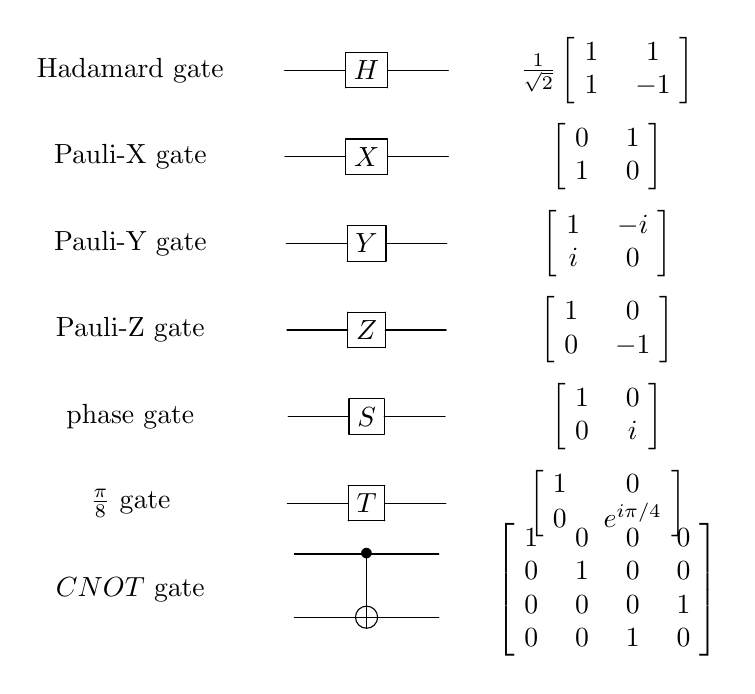
\begin{tikzpicture}
	% $CNOT$
	\node at (7,0){	$CNOT$ gate };
	\node at (10,0){	
		\Qcircuit @C=2.2em @R=1.75em {
		 & \ctrl{1}  & \qw 	 \\
		 &\targ  	 & \qw   \\	    						 
	}};
	\node at (13,0){\vspace{10em}
				$\begin{bmatrix}
					\ 1\ & 0\ & 0\ & 0\ \\
					\ 0\ & 1\ & 0\ & 0\ \\
					\ 0\ & 0\ & 0\ & 1\ \\
					\ 0\ & 0\ & 1\ & 0\ 
				\end{bmatrix}$
	};

		% T
\node at (7,1.1){	$\frac{\pi}{8}$ gate };
\node at (10,1.1){	\Qcircuit @C=2.2em @R=1.75em {
	 & \gate{T}  & \qw 	 \\						 
}};
\node at (13,1.1){\vspace{10em}
			$\begin{bmatrix}
				\ 1\ & 0\  \\
				\ 0\ & e^{i\pi/4}\ \\
			\end{bmatrix}$
};
% phase gate
\node at (7,2.2){	phase gate };
\node at (10,2.2){	
	\Qcircuit @C=2.2em @R=1.75em {
	 & \gate{S}  & \qw 	 \\						 
}};
\node at (13,2.2){\vspace{10em}
			$\begin{bmatrix}
				\ 1\ & 0\  \\
				\ 0\ & i\ \\
			\end{bmatrix}$
};

% Z gate
\node at (7,3.3){	Pauli-Z gate };
\node at (10,3.3){	
	\Qcircuit @C=2.2em @R=1.75em {
	 & \gate{Z}  & \qw 	 \\						 
}};
\node at (13,3.3){\vspace{10em}
			$\begin{bmatrix}
				\ 1\ & 0\  \\
				\ 0\ & -1\ \\
			\end{bmatrix}$
};

% Y gate
\node at (7,4.4){	Pauli-Y gate };
\node at (10,4.4){	
	\Qcircuit @C=2.2em @R=1.75em {
	 & \gate{Y}  & \qw 	 \\						 
}};
\node at (13,4.4){\vspace{10em}
			$\begin{bmatrix}
				\ 1\ & -i\  \\
				\ i\ & 0\ \\
			\end{bmatrix}$
};
% X gate
\node at (7,5.5){	Pauli-X gate };
\node at (10,5.5){	
	\Qcircuit @C=2.2em @R=1.75em {
	 & \gate{X}  & \qw 	 \\						 
}};
\node at (13,5.5){\vspace{10em}
			$\begin{bmatrix}
				\ 0\ & 1\  \\
				\ 1\ & 0\ \\
			\end{bmatrix}$
};
% H
	% IBM Q20
	\node at (7,6.6){	Hadamard gate };
	\node at (10,6.6){	\Qcircuit @C=2.2em @R=1.75em {
		 & \gate{H}  & \qw 	 \\  						 
	}};
	\node at (13,6.6){\vspace{10em}
				$\frac{1}{\sqrt{2}}\begin{bmatrix}
					\ 1\ & 1\ \\
					\ 1\ & -1\ 
				\end{bmatrix}$
	};
\end{tikzpicture}
\end{center}

\caption{The symbols of common quantum gates and their matrices}\label{common_gates}
\end{figure}	 

}

\subsection{Quantum Circuit}
A quantum logical circuit $LC$ (see Fig.~\ref{OriginalCircuit})
consists of quantum gates interconnected by quantum wires~\cite{Daei2020}.
A quantum wire is a mechanism for moving quantum data from one location to another.
Each line represents a qubit, and the gate operation on the line acts on the corresponding qubit.
The width $w$ of a circuit refers to the number of qubits in the circuit.
The depth $d$ of a circuit refers to the number of layers executed in parallel.
The directed acyclic graph (see Fig.~\ref{DAG}) of a circuit is obtained by parallelizing and layering the circuit by topological sorting.
In this paper, circuits with a depth less than 100 are called small-sized circuits,
circuits with a depth greater than 1000 are called large-sized circuits,
and the rest are medium-sized circuits.
The execution order of a quantum logical circuit graph is from left to right.
The depth of the circuit (see Fig.~\ref{OriginalCircuit}) is 6, and the width is 5.
It is unnecessary to consider single quantum gates in circuit transformation since the qubit is \emph{local}~\cite{2013Optimization}.
Architecture graph $\mathcal{AG}_{L}$ is generated by regarding qubits in $LC$ as nodes $V$ and 2-qubit gates as edges $E$.
Our initial mapping tries to find subgraphs isomorphic to the logical architecture graph ($LAG$) on the physical architecture graph ($PAG$).

\begin{figure}[h!] 
	\begin{center}
		  {\scalefont{1.0}
	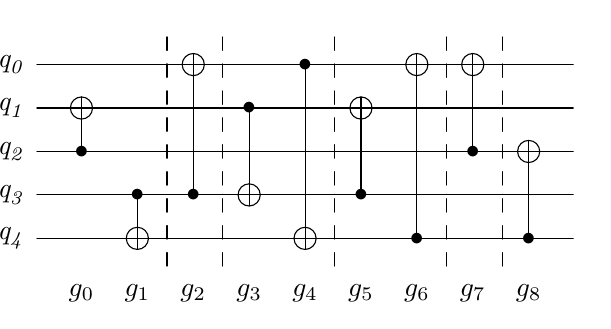
\begin{tikzpicture}
		% \draw[help lines] (0,0) grid (11,7);
		% IBM Q20
		\node at (5.5,5){  \Qcircuit @C=1.2em @R=0.75em {
			\lstick{\textit{q}_\textit{0}}   &  \qw 				&   \qw  \barrier{4}&\targ 	\barrier{4}	&\qw      		&\ctrl{4}\barrier{4}&   \qw		&\targ\barrier{4} &\targ  \barrier{4}&\qw  &  \qw       \\
			\lstick{\textit{q}_\textit{1}}   &   \targ      		&   \qw      		&   \qw      		&   \ctrl{2} 	&   \qw      	&   \targ    	&   \qw      	&   \qw       	&   \qw   		&  \qw       \\
			\lstick{\textit{q}_\textit{2}}   &   \ctrl{-1}  		&   \qw      		&   \qw      		&   \qw      	&   \qw      	&   \qw      	&   \qw     	&   \ctrl{-2} 	&   \targ       &  \qw       \\
			\lstick{\textit{q}_\textit{3}}   &\qw					&   \ctrl{1}   		&   \ctrl{-3} 		&   \targ    	&   \qw      	&   \ctrl{-2}	&   \qw      	&   \qw       	&   \qw        	&  \qw         \\
			\lstick{\textit{q}_\textit{4}}   &		\qw				& \targ				& \qw 				&   \qw      	&   \targ    	&   \qw      	&   \ctrl{-4}  	& 	\qw     	&   \ctrl{-2} 	&   \qw			\\
							  &\dstick{g_{0}}		&\dstick{g_{1}}		&\dstick{g_{2}}		&\dstick{g_{3}}	&\dstick{g_{4}} &\dstick{g_{5}} &\dstick{g_{6}} &\dstick{g_{7}} &\dstick{g_{8}}	&   		\\		 
							 &						&					&				&       		& 				& 				& 				&				&   				 
							 }};
	\end{tikzpicture}
	}
	\end{center}					 
	\caption{Original circuit}
	\label{OriginalCircuit}	
	 \end{figure}

	 \begin{figure}[h!] 
		\begin{center}
	{\scalefont{1}
		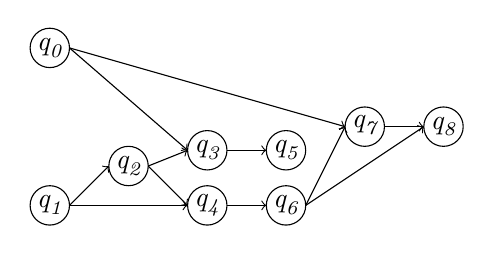
\begin{tikzpicture}							 
	\draw [black,  thin] (3,1) circle [radius=0.25];
	\draw [black,  thin] (3,3) circle [radius=0.25];
	\draw [black,  thin] (4,1.5) circle [radius=0.25];
	\draw [black,  thin] (5,1) circle [radius=0.25];
	\draw [black,  thin] (5,1.7) circle [radius=0.25];
	\draw [black,  thin] (6,1.7) circle [radius=0.25];
	\draw [black,  thin] (6,1) circle [radius=0.25];
	\draw [black,  thin] (7,2) circle [radius=0.25];
	\draw [black,  thin] (8,2) circle [radius=0.25];
	% label
	\node at (3,1) {$\textit{q}_\textit{1}$};
	\node at (3,3) {$\textit{q}_\textit{0}$};
	\node at (4,1.5) {$\textit{q}_\textit{2}$};
	\node at (5,1){$\textit{q}_\textit{4}$};
	\node at (5,1.7) {$\textit{q}_\textit{3}$};
	\node at (6,1.7){$\textit{q}_\textit{5}$};
	\node at (6,1) {$\textit{q}_\textit{6}$};
	\node at (7,2) {$\textit{q}_\textit{7}$};
	\node at (8,2) {$\textit{q}_\textit{8}$};

	% q1
	\draw [->, thin] (3.25,1) -- (3.75,1.5);
	\draw [->, thin] (3.25,1) -- (4.75,1);
	% q0
	\draw [->, thin] (3.25,3) -- (4.75,1.7);
	\draw [->, thin] (3.25,3) -- (6.75,2);
	% q2
	\draw [->, thin] (4.25,1.5) -- (4.75,1);
	\draw [->, thin] (4.25,1.5) -- (4.75,1.7);
	% q3
	\draw [->, thin] (5.25,1.7) -- (5.75,1.7);
	% q4
	\draw [->, thin] (5.25,1) -- (5.75,1);
	% q6
	\draw [->, thin] (6.25,1) -- (7.75,2);
	\draw [->, thin] (6.25,1) -- (6.75,2);
	% q7
	\draw [->, thin] (7.25,2) -- (7.75,2);
	\end{tikzpicture}
}
\end{center}
	\caption{The directed acyclic graph ($DAG$) of original circuit in Fig.~\ref{OriginalCircuit}}
	\label{DAG}
\end{figure}

\begin{figure}[h!]
	\begin{center}
		{\scalefont{1}
	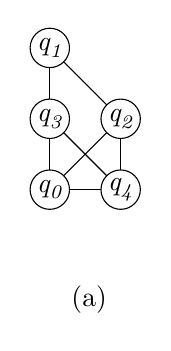
\begin{tikzpicture}
		% \tikzstyle{every node}=[font=\small,scale=0.9]

		\node at (0.5,0){(a)};
            % Q20
            \draw [black, thin] (0,1.4) circle [radius=0.25];
            \draw [-,thin] (0.25,1.4) -- (0.65,1.4);
            \draw [black, thin] (0.9,1.4) circle [radius=0.25];
            % label
            \node at (0,1.4) {$\textit{q}_\textit{0}$};
            \node at (0.9,1.4){$\textit{q}_\textit{4}$};
            % |
            \draw [-,thin] (0,1.65) -- (0,2.05);
            \draw [-,thin] (0.9,1.65)-- (0.9,2.05);
        
            \draw [black, thin] (0,2.3) circle [radius=0.25];
        
            \draw [black, thin] (0.9,2.3) circle [radius=0.25];
            % label
            \node at (0,2.3) {$\textit{q}_\textit{3}$};
            \node at (0.9,2.3){$\textit{q}_\textit{2}$};
            % |
            \draw [-,thin] (0,2.55) -- (0,2.95);
        
            \draw [black, thin] (0,3.2) circle [radius=0.25];
            \draw [-,thin] (0.175,3.025) -- (0.725,2.475);
            % label
            \node at (0,3.2) {$\textit{q}_\textit{1}$};
        
            %x
			\draw [-,thin] (0.175,2.125) -- (0.725,1.575);
			\draw [-,thin] (0.175,1.575) -- (0.725,2.125);
			\label{LLAG}
			\end{tikzpicture}
			}
			\qquad   \qquad
			{\scalefont{0.8}
			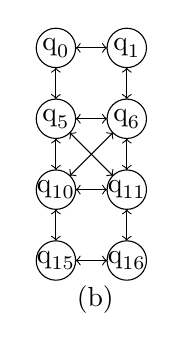
\begin{tikzpicture}
            
                % IBM Q20
            \node at (0.5,0){(b)};
            % Q20
            \draw [black, thin] (0,0.5) circle [radius=0.25];
            \draw [<->,thin] (0.25,0.5) -- (0.65,0.5);
            \draw [black, thin] (0.9,0.5) circle [radius=0.25];
        
            \node at (0,0.5) {$\textup{q}_\textup{15}$};
            \node at (0.9,0.5){$\textup{q}_\textup{16}$};
            % |
            \draw [<->,thin] (0,0.75) -- (0,1.15);
            \draw [<->,thin] (0.9,0.75) -- (0.9,1.15);
        
            \draw [black, thin] (0,1.4) circle [radius=0.25];
            \draw [<->,thin] (0.25,1.4) -- (0.65,1.4);
            \draw [black, thin] (0.9,1.4) circle [radius=0.25];
            % label
            \node at (0,1.4) {$\textup{q}_\textup{10}$};
            \node at (0.9,1.4){$\textup{q}_\textup{11}$};
            % |
            \draw [<->,thin] (0,1.65) -- (0,2.05);
            \draw [<->,thin] (0.9,1.65)-- (0.9,2.05);
        
            \draw [black, thin] (0,2.3) circle [radius=0.25];
            \draw [<->,thin] (0.25,2.3) -- (0.65,2.3);
            \draw [black, thin] (0.9,2.3) circle [radius=0.25];
            % label
            \node at (0,2.3) {$\textup{q}_\textup{5}$};
            \node at (0.9,2.3){$\textup{q}_\textup{6}$};
            % |
            \draw [<->,thin] (0,2.55) -- (0,2.95);
            \draw [<->,thin] (0.9,2.55)-- (0.9,2.95);
        
            \draw [black, thin] (0,3.2) circle [radius=0.25];
            \draw [<->,thin] (0.25,3.2) -- (0.65,3.2);
            \draw [black, thin] (0.9,3.2) circle [radius=0.25];
            % label
            \node at (0,3.2) {$\textup{q}_\textup{0}$};
            \node at (0.9,3.2){$\textup{q}_\textup{1}$};
        
            %x
        
            \draw [<->,thin] (0.175,2.125) -- (0.725,1.575);
			\draw [<->,thin] (0.175,1.575) -- (0.725,2.125);
			\label{PPAG}
	\end{tikzpicture}
			}
\end{center}
	
	\caption{(a) The architecture graph of original circuit in Fig.~\ref{OriginalCircuit}. (b) The partial architecture graph of IBM Q20 }
	\label{LAGPAG}
\end{figure}
	
\begin{figure}[h!] 				
	\centerline{ 
\Qcircuit @C=1.2em @R=1.5em {
							 &  \ctrl{1}  		&     \qw \\
							 &   \targ      		&       \qw   \\	 
							&					&      						 
					}
					  \qquad    \qquad
  \Qcircuit @C=1.2em @R=0.75em {
	 &   \gate{H}  		&\targ 			&\gate{H}     	&    \qw  	 \\
	 &   \gate{H}      	&\ctrl{-1}      &\gate{H} 		&   \qw 	    \\	 
	&					&				& 				&						 
					  }
  }

  \caption{Transformation of gate direction}
  \label{Transformate}
\end{figure}
\begin{figure}[h!] 				
   \centerline{ 
					\Qcircuit @C=1.2em @R=2.05em {
											\lstick{\textit{q}_\textit{0}} &  \qswap  				&    \rstick{\textit{q}_\textit{1}} \qw \\
											\lstick{\textit{q}_\textit{1}} &   \qswap\qwx	   		&     \rstick{\textit{q}_\textit{0}}  \qw   \\	 
																					&					&      						 
										}
										\qquad    \qquad
\Qcircuit @C=1.2em @R=1.22em {
					   \lstick{\textit{q}_\textit{0}} 	&  \ctrl{1}  		&  \targ  		&  \ctrl{1}  		&    \rstick{\textit{q}_\textit{1}} \qw \\
					   \lstick{\textit{q}_\textit{1}} 	&   \targ      		&  \ctrl{-1}    &   \targ      		&     \rstick{\textit{q}_\textit{0}}  \qw   \\	 
										&					&				&					&      						 
				   }
					 \qquad    \qquad
 \Qcircuit @C=1.2em @R=0.75em {
	\lstick{\textit{q}_\textit{0}}  &  \ctrl{1}  		&   \gate{H}  		&\ctrl{1} 			&\gate{H}     	&\ctrl{1}			&    \rstick{\textit{q}_\textit{1}}\qw  	 \\
	\lstick{\textit{q}_\textit{1}}  &   \targ      		&   \gate{H}      	&   \targ      		&\gate{H} 		&\targ      		&    \rstick{\textit{q}_\textit{0}}\qw 	    \\	 
					&					&					&					&       		& 					&						 
					 }
 }

   \caption{Decomposition of a SWAP gate	   }
   \label{Decomposition}
 \end{figure}

\subsection{Architectures}
We mainly discuss the physical circuits of IBM Q series.
Let $\mathcal{\mathcal{AG}_{P}}=(V_{P}, E_{P})$ denote the architecture graph of the physical circuit,
where $V_{P}$ denotes the physical qubit set and $E_{P}$ represents the directed edge set that the $CNOT$ gates.
Fig.~\ref{IBM} (a) and (b) are $PAG$ of the 5-qubit of IBM QX2,
(c) and (d) are $PAG$ of 16$-$qubit of IBM QX3,
and (e) are the $PAG$ of IBM Q20.
An arrow in the figure indicates that the qubit at the beginning of the arrow can control the qubit at the end of the arrow,
and the 2-qubit gate operations can only be performed between qubits with edges connected.
IBM physical circuit only supports single quantum gates and $CNOT$ gates between two adjacent qubits.
Fig.~\ref{LAGPAG}(a) is the logical architecture of the original circuit of Fig.~\ref{OriginalCircuit},
and Fig.~\ref{LAGPAG}(b) is the partial architecture graph of IBM Q20. 

\begin{figure}
	{
	\scalefont{0.8}
	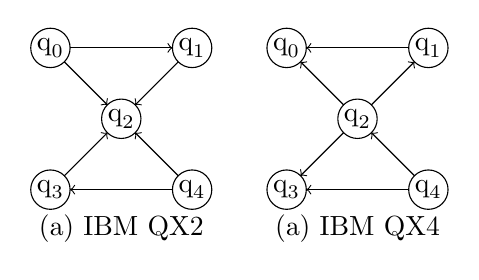
\begin{tikzpicture}
	% \draw[help lines] (0,0) grid (11,3);
		% IBM QX2
	\node at (1.8,0.4){(a) IBM QX2};
	\node at (4.8,0.4){(a) IBM QX4};
	% label
	\node at (0.9,2.7){$\textup{q}_\textup{0}$};
	\draw [black, thin] (0.9,2.7) circle [radius=0.25];
	\node at (2.7,2.7){$\textup{q}_\textup{1}$};
	\draw [black, thin] (2.7,2.7) circle [radius=0.25];
	\node at (1.8,1.8){$\textup{q}_\textup{2}$};
	\draw [black, thin] (1.8,1.8)circle [radius=0.25];
	\node at (0.9,0.9){$\textup{q}_\textup{3}$};
	\draw [black, thin] (0.9,0.9) circle [radius=0.25];
	\node at (2.7,0.9){$\textup{q}_\textup{4}$};
	\draw [black, thin] (2.7,0.9) circle [radius=0.25];

	
	% -
	\draw [->,thin] (1.15,2.7) -- (2.45,2.7);
	
	\draw [<-,thin] (1.15,0.9) -- (2.45,0.9);

	%x
	\draw [->,thin] (1.075,2.525) -- (1.625,1.975);
	\draw [->,thin] (2.525,2.525) -- (1.975,1.975);
	\draw [->,thin] (1.075,1.075) -- (1.625,1.625);
	\draw [->,thin] (2.525,1.075) -- (1.975,1.625);

		 
		% label
		\node at (3.9,2.7){$\textup{q}_\textup{0}$};
		\draw [black, thin] (3.9,2.7) circle [radius=0.25];
		\node at (5.7,2.7){$\textup{q}_\textup{1}$};
		\draw [black, thin] (5.7,2.7) circle [radius=0.25];
		\node at (4.8,1.8){$\textup{q}_\textup{2}$};
		\draw [black, thin] (4.8,1.8)circle [radius=0.25];
		\node at (3.9,0.9){$\textup{q}_\textup{3}$};
		\draw [black, thin] (3.9,0.9) circle [radius=0.25];
		\node at (5.7,0.9){$\textup{q}_\textup{4}$};
		\draw [black, thin] (5.7,0.9) circle [radius=0.25];
		
		% -
		\draw [<-,thin] (4.15,2.7) -- (5.45,2.7);
		
		\draw [<-,thin] (4.15,0.9) -- (5.45,0.9);

		\draw [<-,thin] (4.075,2.525) -- (4.625,1.975);
		\draw [<-,thin] (5.525,2.525) -- (4.975,1.975);
		\draw [<-,thin] (4.075,1.075) -- (4.625,1.625);
		\draw [->,thin] (5.525,1.075) -- (4.975,1.625);
	
	\end{tikzpicture}
}
\\
{
	\scalefont{0.8}
		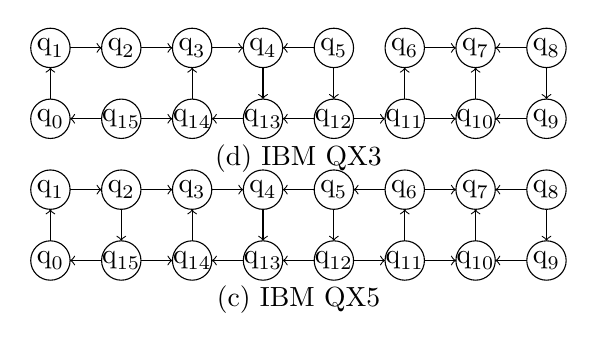
\begin{tikzpicture}
			
	\node at (3.15,0){(c) IBM QX5};
	\node at (3.15,1.8){(d) IBM QX3};
		%QX5
		%-
	\draw [black, thin] (0,2.3) circle [radius=0.25];
	\draw [<-,thin] (0.25,2.3) -- (0.65,2.3);
	\draw [black, thin] (0.9,2.3) circle [radius=0.25];
	\draw [->,thin] (1.15,2.3) -- (1.55,2.3);
	\draw [black, thin] (1.8,2.3) circle [radius=0.25];
	\draw [<-,thin] (2.05,2.3) -- (2.45,2.3);
	\draw [black, thin] (2.7,2.3) circle [radius=0.25];
	\draw [<-,thin] (2.95,2.3) -- (3.35,2.3);
	\draw [black, thin] (3.6,2.3) circle [radius=0.25];
	\draw [->,thin] (3.85,2.3) -- (4.25,2.3);
	\draw [black, thin] (4.5,2.3) circle [radius=0.25];
	\draw [->,thin] (4.75,2.3) -- (5.15,2.3);
	\draw [black, thin] (5.4,2.3) circle [radius=0.25];
	\draw [<-,thin] (5.65,2.3) -- (6.05,2.3);
	\draw [black, thin] (6.3,2.3) circle [radius=0.25];

	% |
	\draw [->,thin] (0,2.55) -- (0,2.95);
	\draw [->,thin] (1.8,2.55) -- (1.8,2.95);
	\draw [<-,thin] (2.7,2.55) -- (2.7,2.95);
	\draw [<-,thin] (3.6,2.55) -- (3.6,2.95);
	\draw [->,thin] (4.5,2.55) -- (4.5,2.95);
	\draw [->,thin] (5.4,2.55) -- (5.4,2.95);
	\draw [<-,thin] (6.3,2.55) -- (6.3,2.95);
	%-
\draw [black, thin] (0,3.2) circle [radius=0.25];
\draw [->,thin] (0.25,3.2) -- (0.65,3.2);
\draw [black, thin] (0.9,3.2) circle [radius=0.25];
\draw [->,thin] (1.15,3.2) -- (1.55,3.2);
\draw [black, thin] (1.8,3.2) circle [radius=0.25];
\draw [->,thin] (2.05,3.2) -- (2.45,3.2);
\draw [black, thin] (2.7,3.2) circle [radius=0.25];
\draw [<-,thin] (2.95,3.2) -- (3.35,3.2);
\draw [black, thin] (3.6,3.2) circle [radius=0.25];

\draw [black, thin] (4.5,3.2) circle [radius=0.25];
\draw [->,thin] (4.75,3.2) -- (5.15,3.2);
\draw [black, thin] (5.4,3.2) circle [radius=0.25];
\draw [<-,thin] (5.65,3.2) -- (6.05,3.2);
\draw [black, thin] (6.3,3.2) circle [radius=0.25];
	
	% label
	\node at (0,0.5){$\textup{q}_\textup{0}$};
	\node at (0.9,0.5){$\textup{q}_\textup{15}$};
	\node at (1.8,0.5){$\textup{q}_\textup{14}$};
	\node at (2.7,0.5){$\textup{q}_\textup{13}$};
	\node at (3.6,0.5){$\textup{q}_\textup{12}$};
	\node at (4.5,0.5){$\textup{q}_\textup{11}$};
	\node at (5.4,0.5){$\textup{q}_\textup{10}$};
	\node at (6.3,0.5){$\textup{q}_\textup{9}$};

	\node at (0,1.4){$\textup{q}_\textup{1}$};
	\node at (0.9,1.4){$\textup{q}_\textup{2}$};
	\node at (1.8,1.4){$\textup{q}_\textup{3}$};
	\node at (2.7,1.4){$\textup{q}_\textup{4}$};
	\node at (3.6,1.4){$\textup{q}_\textup{5}$};
	\node at (4.5,1.4){$\textup{q}_\textup{6}$};
	\node at (5.4,1.4){$\textup{q}_\textup{7}$};
	\node at (6.3,1.4){$\textup{q}_\textup{8}$};

		%QX5
		%-
		\draw [black, thin] (0,0.5) circle [radius=0.25];
		\draw [<-,thin] (0.25,0.5) -- (0.65,0.5);
		\draw [black, thin] (0.9,0.5) circle [radius=0.25];
		\draw [->,thin] (1.15,0.5) -- (1.55,0.5);
		\draw [black, thin] (1.8,0.5) circle [radius=0.25];
		\draw [<-,thin] (2.05,0.5) -- (2.45,0.5);
		\draw [black, thin] (2.7,0.5) circle [radius=0.25];
		\draw [<-,thin] (2.95,0.5) -- (3.35,0.5);
		\draw [black, thin] (3.6,0.5) circle [radius=0.25];
		\draw [->,thin] (3.85,0.5) -- (4.25,0.5);
		\draw [black, thin] (4.5,0.5) circle [radius=0.25];
		\draw [->,thin] (4.75,0.5) -- (5.15,0.5);
		\draw [black, thin] (5.4,0.5) circle [radius=0.25];
		\draw [<-,thin] (5.65,0.5) -- (6.05,0.5);
		\draw [black, thin] (6.3,0.5) circle [radius=0.25];
	
		% |
		\draw [->,thin] (0,0.75) -- (0,1.15);
		\draw [<-,thin] (0.9,0.75) -- (0.9,1.15);
		\draw [->,thin] (1.8,0.75) -- (1.8,1.15);
		\draw [<-,thin] (2.7,0.75) -- (2.7,1.15);
		\draw [<-,thin] (3.6,0.75) -- (3.6,1.15);
		\draw [->,thin] (4.5,0.75) -- (4.5,1.15);
		\draw [->,thin] (5.4,0.75) -- (5.4,1.15);
		\draw [<-,thin] (6.3,0.75) -- (6.3,1.15);
		%-
	\draw [black, thin] (0,1.4) circle [radius=0.25];
	\draw [->,thin] (0.25,1.4) -- (0.65,1.4);
	\draw [black, thin] (0.9,1.4) circle [radius=0.25];
	\draw [->,thin] (1.15,1.4) -- (1.55,1.4);
	\draw [black, thin] (1.8,1.4) circle [radius=0.25];
	\draw [->,thin] (2.05,1.4) -- (2.45,1.4);
	\draw [black, thin] (2.7,1.4) circle [radius=0.25];
	\draw [<-,thin] (2.95,1.4) -- (3.35,1.4);
	\draw [black, thin] (3.6,1.4) circle [radius=0.25];
	\draw [<-,thin] (3.85,1.4) -- (4.25,1.4);
	\draw [black, thin] (4.5,1.4) circle [radius=0.25];
	\draw [->,thin] (4.75,1.4) -- (5.15,1.4);
	\draw [black, thin] (5.4,1.4) circle [radius=0.25];
	\draw [<-,thin] (5.65,1.4) -- (6.05,1.4);
	\draw [black, thin] (6.3,1.4) circle [radius=0.25];
		
		% label
		\node at (0,2.3){$\textup{q}_\textup{0}$};
		\node at (0.9,2.3){$\textup{q}_\textup{15}$};
		\node at (1.8,2.3){$\textup{q}_\textup{14}$};
		\node at (2.7,2.3){$\textup{q}_\textup{13}$};
		\node at (3.6,2.3){$\textup{q}_\textup{12}$};
		\node at (4.5,2.3){$\textup{q}_\textup{11}$};
		\node at (5.4,2.3){$\textup{q}_\textup{10}$};
		\node at (6.3,2.3){$\textup{q}_\textup{9}$};
	
		\node at (0,3.2){$\textup{q}_\textup{1}$};
		\node at (0.9,3.2){$\textup{q}_\textup{2}$};
		\node at (1.8,3.2){$\textup{q}_\textup{3}$};
		\node at (2.7,3.2){$\textup{q}_\textup{4}$};
		\node at (3.6,3.2){$\textup{q}_\textup{5}$};
		\node at (4.5,3.2){$\textup{q}_\textup{6}$};
		\node at (5.4,3.2){$\textup{q}_\textup{7}$};
		\node at (6.3,3.2){$\textup{q}_\textup{8}$};
	\end{tikzpicture}
}
{\scalefont{0.8}
	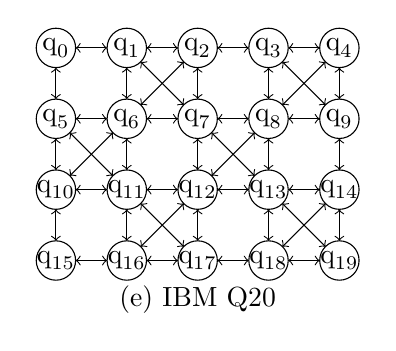
\begin{tikzpicture}
	
		% IBM Q20
		\node at (1.8,0){(e) IBM Q20};
	% Q20
	\draw [black, thin] (0,0.5) circle [radius=0.25];
	\draw [<->,thin] (0.25,0.5) -- (0.65,0.5);
	\draw [black, thin] (0.9,0.5) circle [radius=0.25];
	\draw [<->,thin] (1.15,0.5) -- (1.55,0.5);
	\draw [black, thin] (1.8,0.5) circle [radius=0.25];
	\draw [<->,thin] (2.05,0.5) -- (2.45,0.5);
	\draw [black, thin] (2.7,0.5) circle [radius=0.25];
	\draw [<->,thin] (2.95,0.5) -- (3.35,0.5);
	\draw [black, thin] (3.6,0.5) circle [radius=0.25];

	\node at (0,0.5) {$\textup{q}_\textup{15}$};
	\node at (0.9,0.5){$\textup{q}_\textup{16}$};
	\node at (1.8,0.5){$\textup{q}_\textup{17}$};
	\node at (2.7,0.5){$\textup{q}_\textup{18}$};
	\node at (3.6,0.5){$\textup{q}_\textup{19}$};
	% |
	\draw [<->,thin] (0,0.75) -- (0,1.15);
	\draw [<->,thin] (0.9,0.75) -- (0.9,1.15);
	\draw [<->,thin] (1.8,0.75) -- (1.8,1.15);
	\draw [<->,thin] (2.7,0.75) -- (2.7,1.15);
	\draw [<->,thin] (3.6,0.75) -- (3.6,1.15);

	\draw [black, thin] (0,1.4) circle [radius=0.25];
	\draw [<->,thin] (0.25,1.4) -- (0.65,1.4);
	\draw [black, thin] (0.9,1.4) circle [radius=0.25];
	\draw [<->,thin] (1.15,1.4) -- (1.55,1.4);
	\draw [black, thin] (1.8,1.4)circle [radius=0.25];
	\draw [<->,thin] (2.05,1.4) -- (2.45,1.4);
	\draw [black, thin] (2.7,1.4) circle [radius=0.25];
	\draw [<->,thin] (2.95,1.4) -- (3.35,1.4);
	\draw [black, thin] (3.6,1.4) circle [radius=0.25];
	% label
	\node at (0,1.4) {$\textup{q}_\textup{10}$};
	\node at (0.9,1.4){$\textup{q}_\textup{11}$};
	\node at (1.8,1.4){$\textup{q}_\textup{12}$};
	\node at (2.7,1.4){$\textup{q}_\textup{13}$};
	\node at (3.6,1.4){$\textup{q}_\textup{14}$};
	% |
	\draw [<->,thin] (0,1.65) -- (0,2.05);
	\draw [<->,thin] (0.9,1.65)-- (0.9,2.05);
	\draw [<->,thin] (1.8,1.65) -- (1.8,2.05);
	\draw [<->,thin] (2.7,1.65) -- (2.7,2.05);
	\draw [<->,thin] (3.6,1.65) -- (3.6,2.05);

	\draw [black, thin] (0,2.3) circle [radius=0.25];
	\draw [<->,thin] (0.25,2.3) -- (0.65,2.3);
	\draw [black, thin] (0.9,2.3) circle [radius=0.25];
	\draw [<->,thin] (1.15,2.3) -- (1.55,2.3);
	\draw [black, thin] (1.8,2.3)circle [radius=0.25];
	\draw [<->,thin] (2.05,2.3) -- (2.45,2.3);
	\draw [black, thin] (2.7,2.3) circle [radius=0.25];
	\draw [<->,thin] (2.95,2.3) -- (3.35,2.3);
	\draw [black, thin] (3.6,2.3) circle [radius=0.25];
	% label
	\node at (0,2.3) {$\textup{q}_\textup{5}$};
	\node at (0.9,2.3){$\textup{q}_\textup{6}$};
	\node at (1.8,2.3){$\textup{q}_\textup{7}$};
	\node at (2.7,2.3){$\textup{q}_\textup{8}$};
	\node at (3.6,2.3){$\textup{q}_\textup{9}$};
	% |
	\draw [<->,thin] (0,2.55) -- (0,2.95);
	\draw [<->,thin] (0.9,2.55)-- (0.9,2.95);
	\draw [<->,thin] (1.8,2.55) -- (1.8,2.95);
	\draw [<->,thin] (2.7,2.55) -- (2.7,2.95);
	\draw [<->,thin] (3.6,2.55) -- (3.6,2.95);

	\draw [black, thin] (0,3.2) circle [radius=0.25];
	\draw [<->,thin] (0.25,3.2) -- (0.65,3.2);
	\draw [black, thin] (0.9,3.2) circle [radius=0.25];
	\draw [<->,thin] (1.15,3.2) -- (1.55,3.2);
	\draw [black, thin] (1.8,3.2)circle [radius=0.25];
	\draw [<->,thin] (2.05,3.2) -- (2.45,3.2);
	\draw [black, thin] (2.7,3.2) circle [radius=0.25];
	\draw [<->,thin] (2.95,3.2) -- (3.35,3.2);
	\draw [black, thin] (3.6,3.2) circle [radius=0.25];
	% label
	\node at (0,3.2) {$\textup{q}_\textup{0}$};
	\node at (0.9,3.2){$\textup{q}_\textup{1}$};
	\node at (1.8,3.2){$\textup{q}_\textup{2}$};
	\node at (2.7,3.2){$\textup{q}_\textup{3}$};
	\node at (3.6,3.2){$\textup{q}_\textup{4}$};

	%x
	\draw [<->,thin] (1.075,0.675) -- (1.625,1.225);
	\draw [<->,thin] (1.075,1.225) -- (1.625,0.675);
	\draw [<->,thin] (2.875,0.675) -- (3.425,1.225);
	\draw [<->,thin] (2.875,1.225) -- (3.425,0.675);
		%3
	\draw [<->,thin] (1.075,2.475) -- (1.625,3.025);
	\draw [<->,thin] (1.075,3.025) -- (1.625,2.475);
	\draw [<->,thin] (2.875,2.475) -- (3.425,3.025);
	\draw [<->,thin] (2.875,3.025) -- (3.425,2.475);
		% 2
	\draw [<->,thin] (0.175,2.125) -- (0.725,1.575);
	\draw [<->,thin] (0.175,1.575) -- (0.725,2.125);
	\draw [<->,thin] (1.975,2.125) -- (2.525,1.575);
	\draw [<->,thin] (1.975,1.575) -- (2.525,2.125);
	\end{tikzpicture}
}
\caption{IBM QX architectures}
\label{IBM}
\end{figure}


\section{Problem Analysis}
\label{Problem Analysis}

\paragraph{Problem in qubit Mapping}
Single qubit gates and $CNOT$ gates are used as basic gates since they are commonly used to implement any quantum circuit supported by the IBM QX architecture. Before circuit transformation, the circuit should be simplified to a circuit with only single quantum gates and $CNOT$ gates~\cite{2005Mttnen,1995Barenco}. We insert auxiliary gates (see Fig.~\ref{Decomposition}) so that two non-adjacent qubits can move to adjacent positions or change direction between two adjacent qubits (see Fig.~\ref{Transformate}). The introduction of auxiliary gates may lead to errors, leading to a large deviation between the final results and the actual situation. The quantum system is easy to interact with the surrounding environment, resulting in errors. In the NISQ era, quantum error correction is difficult to achieve. Due to the decoherence problem of quantum bits, the quantum operation needs to be completed in a coherent period, and the time of quantum bits in the coherent state is short. Therefore, it is necessary to improve the parallelism of qubits as much as possible to minimize the depth of the quantum circuit. This is the focus of this paper. We hope to find a circuit transformation algorithm to make the output circuit with the minimum number of auxiliary gates and the circuit depth in an acceptable amount of time.

Given the logical circuit $LC$, physical structure $\mathcal{AG}_{P}$, 
and an initial mapping $\tau$, $CNOT$ gate $g=\left \langle \textit{q}_\textit{i},\textit{q}_\textit{j}\right \rangle $, 
$\left \langle\tau(\textit{q}_\textit{i}),\tau(\textit{q}_\textit{j})\right \rangle $ 
is a directed edge on $\mathcal{AG}_{P}$, if gate $G$ is executable.

\begin{example}
	Fig.~\ref{LAGPAG} (a) is the logical structure of Fig.~\ref{OriginalCircuit}, 
	Fig.~\ref{LAGPAG} (b) is the partial architecture graph of IBM Q20, an initial mapping is 
	$\tau=\{\textit{q}_\textit{0}\rightarrow  \textup{q}_{\textup{10}},\ \textit{q}_\textit{1}\rightarrow \textup{q}_{\textup{0}},\ 
	\textit{q}_\textit{2}\rightarrow  \textup{q}_{\textup{6}},\ \textit{q}_\textit{3}\rightarrow  \textup{q}_{\textup{5}},\ \textit{q}_\textit{4}\rightarrow  \textup{q}_{\textup{11}}\}$.
	$g_{0}=\left \langle \textit{q}_\textit{2},\textit{q}_\textit{1}\right \rangle $ is not executable, since 
	$\left \langle \tau(\textit{q}_\textit{2}),\tau(\textit{q}_\textit{1})\right \rangle =\left \langle \textup{q}_{\textup{6}},\textup{q}_{\textup{0}}\right \rangle $ does not  exists in $\mathcal{AG}_{P}$.
	But $g_{3}=\left \langle \textit{q}_\textit{1},\textit{q}_\textit{3}\right \rangle $ is executable, since 
	$\left \langle \tau(\textit{q}_\textit{1}),\tau(\textit{q}_\textit{3})\right \rangle =\left \langle \textup{q}_{\textup{0}},\textup{q}_{\textup{5}}\right \rangle $  exist in $\mathcal{AG}_{P}$.
\end{example}

A quantum circuit transformation problem mainly includes the following four steps, among which the third step of isomorphism and the fourth step of the circuit transformation problem are both NPC~\cite{2018QubitSiraichi}
\begin{figure}[h!] 
	\centering
	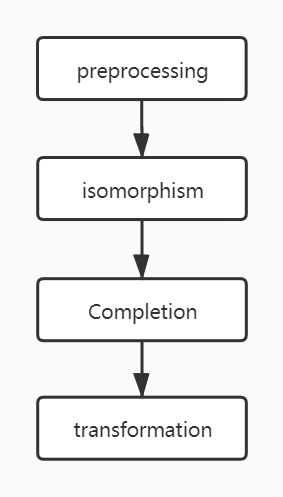
\includegraphics[scale=0.4]{uml.jpg}		 
	\caption{Circuit transformation process}
	\label{processing}	
	 \end{figure}
\begin{enumerate}
	\item \emph{ Preprocess the logical quantum circuit.} 
	It includes extracting the $LAG$ of the circuit, adjusting the life cycle of qubits (this part of the work is done by Zhang~\cite{2019Zhang}),  and calculating the shortest path of the physical circuit.
	\item \emph{Compute isomorphic substructures.}
	It uses the subgraph isomorphism algorithm to find part of the initial mapping, which is done by Sun~\cite{Sun2020}   
	\item \emph{Generate high-quality initial mapping.} We perform mapping completion because the remaining nodes cannot satisfy all isomorphism requirements. According to the connectivity between the unmapped node and the mapped nodes. The unmapped node is mapped to the mapped node's neighborhood, which satisfies the connectivity of part of the structure and reduces the length of the shortest path.  
	\item \emph{Transforming logical circuits to meet physical constraints}
	Circuit transformation problems need to be solved before implementing quantum circuits since quantum algorithms are usually designed without referring to any specific hardware's connectivity constraints. Therefore, circuit transformation forms a necessary stage of any quantum compiler.
\end{enumerate}

\section{Solution}
\label{Solution}
The solution proposed in this paper mainly includes preprocessing, initial mapping, and circuit transformation algorithm based on Tabu Search.
\subsection{Preprocessing}
Before transforming the SWAP circuit based on Tabu Search, we need to preprocess it to get more convenient data to shorten our search time and space. In the preprocessing stage, we adjust the circuit of the input openQASM program to shorten the life cycle of qubits. Then we use Breadth-First Search (BFS) to calculate the shortest distance between each node on the architecture graph.
\subsubsection{Circuit Adjustment}
In order to shorten the life cycle of qubits and improve the parallelism of qubits, we use a layered method to analyze the life cycle of qubits~\cite{2019Zhang} and pack the operations that can be executed in parallel into a $bundle$, forming a layered bundle format.
A conversion method is designed to use the layered bundle format to determine which operations can be moved, which reduces the life cycle of these qubits. The algorithm reduces the error rate of quantum programs by 11\%. On most quantum workloads, the longest qubit lifetime and the average qubit lifetime can be reduced by more than 20\%, and the execution time of some quantum programs can also be reduced.
\subsubsection{Shortest Distance}
Given $PAG$, the shortest distance between two qubits can be calculated. In this paper, the shortest distance matrix $dist[i][j]$ is calculated by $Floyd-Warshall$ algorithm, which represents the shortest distance from $\textup{q}_{\textup{i}}$ to $\textup{q}_{\textup{j}}$, and the distance of each edge is 1. 

For IBM QX2, QX3, QX4, QX5, the SWAP operation needs 7 gates (3 $CNOT$ gates and 4 $H$ gates). Only 4 $H$ gates are needed to change directions between two adjacent qubits. For a $CNOT$ gate $\left \langle  \textit{q}_\textit{i},\textit{q}_\textit{j} \right \rangle $,
Two qubits are mapped to $\textup{q}_{\textup{i}}$ and $\textup{q}_{\textup{j}}$ respectively, with $\ \tau(\textit{q}_\textit{i})=\textup{q}_{\textup{i}},\ \tau(\textit{q}_\textit{j})=\textup{q}_{\textup{j}}$. then the cost of executing $g$ under the shortest distance path is $cost_{cnot}(\textit{q}_\textit{i},\textit{q}_\textit{j})=7 \times( dist[i][j]-1)$. If they move to adjacent positions, but there is no edge from $\textup{q}_{\textup{i}}$ to $\textup{q}_{\textup{j}}$, we need to add 4 $H$ gates to adjust their directions. For IBM Q20, in which all edges are bidirectional, the SWAP operation requires 3 gates (3 $CNOT$ gates), 
and there is no need to change the direction. Thus the cost between them is $cost_{cnot}(\textit{q}_\textit{i},\textit{q}_\textit{j})=3 \times( dist[i][j]-1)$. The time complexity of this step is $O (N^{3})$.
\begin{example}
	Take the QX5 structure as an example. Suppose there is a $CNOT$ gate $g=\left \langle  \textit{q}_\textit{i}, \textit{q}_\textit{j} \right \rangle $, \ $\textit{q}_\textit{i}$ is mapped to $\textup{q}_{1}$,  $\textit{q}_\textit{j}$ is mapped to $\textup{q}_{\textup{14}}$, and the shortest distance between them  is $dist[1][14]=3$. There are 3 shortest paths to move $\textup{q}_{\textup{1}}$ to the adjacent position of 
$\textup{q}_{\textup{14}}$:
$\Pi=\{\pi_{0},\pi_{1},\pi_{2}\}$
$\pi_{0}={\textup{q}_{\textup{1}}\rightarrow \textup{q}_{\textup{2}} \rightarrow \textup{q}_{\textup{3}} \rightarrow \textup{q}_{\textup{14}}}$,
$\pi_{1}={\textup{q}_{\textup{1}}\rightarrow \textup{q}_{\textup{2}} \rightarrow \textup{q}_{\textup{15}} \rightarrow \textup{q}_{\textup{14}}}$,
$\pi_{2}={\textup{q}_{\textup{1}}\rightarrow \textup{q}_{\textup{0}} \rightarrow \textup{q}_{\textup{15}} \rightarrow \textup{q}_{\textup{14}}}$.
Their costs are 
$cost_{\pi_{0}}=18,\ cost_{\pi_{1}}=14,\ cost_{\pi_{2}}=14$, respectively.
\end{example}

\subsubsection{Circuit Layering}
Quantum gates acting on different qubits can be executed in parallel, so we can layer quantum circuits to improve the parallelism of qubits and shorten the life cycle of qubits. Thus, we layer the adjusted circuit, traverse the entire program sequentially, and add gates that can be executed parallel to one layer. Otherwise, a new layer is added. The $CNOT$ gate is represented by $\left \langle  \textit{q}_\textit{i}, \textit{q}_\textit{j} \right \rangle $, $\textit{q}_\textit{i}$ is the control qubit, and $\textit{q}_\textit{j}$ is the target qubit. $L(LC)=\{\mathcal{L}_{0},\mathcal{L}_{1},...,\mathcal{L}_{n}\}$ represents the layered circuit, and $\mathcal{L}_{i} \ (0 \le i \le n) $ represents a quantum gate set that can be executed in parallel. The quantum gate set separated by the dotted line in Fig.~\ref{OriginalCircuit} are the following $\mathcal{L}_{0}=\{g_{0},g_{1}\},\mathcal{L}_{1}=\{g_{2}\},
 \mathcal{L}_{2}=\{g_{3},g_{4}\},\mathcal{L}_{3}=\{g_{5},g_{6}\},\mathcal{L}_{4}=\{g_{7}\},\mathcal{L}_{5}=\{g_{8}\}$.

At the same time, we generate logical circuit architecture graph $\mathcal{AG_{L}}=(V_{L},E_{L})$, which is an undirected graph. $V_{L}$ contains the vertices and the degree of each vertex, and $E_{L}$ represents the set of undirected edges that the $CNOT$ gates can execute.

\subsection{Initial Mapping}
It has been proved that the initial mapping has an important influence on $qubit$  $ assignment$,  and the subgraph isomorphism can be reduced to $qubit$ $ assignment$, so we want to use the subgraph isomorphism algorithm to find an initial mapping that helps to minimize auxiliary gates in transformation stage.

In $PAG$, it is almost impossible to find a subgraph that exactly matched nodes $LAG$, so we hope to find a partial mapping that can maximize the number of match. $SubgraphCompare$~\cite{Sun2020} compares several state-of-the-art subgraph isomorphism algorithm composition. 
It shows that using the filtering and sorting ideas of \emph{GraphQL} algorithm to process candidate nodes, and the local candidates' calculation method \emph{LFTJ} based on set-intersection to enumerate the results is the best. Since $SubgraphCompare$ used in this paper is only suitable for fully connected subgraph isomorphism, there may be no 2-qubit gate operation between one qubit and other qubits in our circuit. The architecture graph formed in this way cannot use $SubgraphCompare$ to generate part of the initial mapping because the subgraph isomorphism will first match the node with the largest degree,  and we hope to minimize the impact on the logical dependency graph. Therefore, we artificially connect the isolating qubit to the qubit with the largest degree in the logical architecture diagram.

We use $SubgraphCompare$ generate partial mappings denoted by $T$. The logical architecture graph  $\mathcal{AG_{L}}$ 
and physical architecture graph $\mathcal{AG_{P}}$ generated by the preprocessing process regard as undirected graph as input. The output of $CSI$ algorithm is a file containing all the isomorphism processes. We only choose the case with the most homogeneous nodes as the $CSI$ result, since only some nodes may be matched during the algorithm. Then we complete the unmapped nodes in the partial mapping based on the connectivity of the nodes or the degree of the nodes. The mapping completion algorithm based on node connectivity is show in Algorithm~\ref{algorithm_initial}.
\begin{algorithm}  
	\label{algorithm_initial}
	\caption{initial mapping algorithm $CSI$}  
	\LinesNumbered  
	\KwIn{$\mathcal{AG_{L}}$: The architecture of logical circuit \\ 
	$\mathcal{AG_{P}}$: The architecture of physical circuit\\
	$T$: A partial mapping set obtained by $SubgraphCompare$  \\
	}
	\KwOut{$result$: A collection of mapping relations between
	 $\mathcal{AG_{L}}$ and $\mathcal{AG_{P}}$}  
	\textbf{Initialize} $result=\emptyset$ ;\\
	$l \leftarrow max_{\tau \in T} \  \tau.length$; \\
	\For{$\tau\in T$}{
		\If{$l=\tau.length$}{
			$result.add(\tau)$;\\
			$Q \leftarrow $ initialing an empty unmapped node queue \\
			$i \leftarrow  1$; \\ 
			\While{$i\leq \tau.length$}{
				\If{$\tau[i]=-1$}{
					$Q \leftarrow {i}$;
				}
				$i \leftarrow i+1$;
			}
			\While{$Q\ is\ not\ empty$}{
				int  $q\_id \leftarrow Q.poll()$;\\
				$targetAdj \leftarrow$ $\mathcal{AG_{P}}.adjacencyMatrix()$; 	\\
				$queryAdj \leftarrow$ $\mathcal{AG_{L}}.adjacencyMatrix()$;	\\
				$cans \leftarrow$ initialing an empty candidate node list \tcp*{sorted by the connectivity of nodes }
				$m \leftarrow 1$; \\
				\While{$m \leq queryAdj[q\_id].length$}{
					\If{$\tau[m]\neq-1$}{
						$cans \leftarrow cans \cup \{ m\}$;	
					}
					$m \leftarrow m+1$;
				}
				\While{$cans\ is\ not\ empty$}{
					$t\_id \leftarrow \tau[cans.first]$; \\
					$k \leftarrow 0$; \\
					$cans \leftarrow cans\backslash cans.first$; \\
					\While{$ k \textless targetAdj[t\_id].length$}{
						\If{  $(targetAdj[t\_id][k]\neq -1\ or\ targetAdj[k][t\_id]  \neq -1)$\\
						  $\ and\ not\ \tau.contains(k)$}{
							 $\tau[q\_id] \leftarrow k$; \\
							 break;
						 }
						  $k \leftarrow k+1$;
					}
					\If{ $k\neq targetAdj[t\_id].length$ }{
						break;
					}
				}
			}
		}
	}
	\end{algorithm}
	
	The input of Algorithm~\ref{algorithm_initial} is a target graph ($\mathcal{AG}_{P}$), query graph ($\mathcal{AG}_{L}$), and the partial mappings $T$. First, we initialize an empty queue $Q$,  which stores unmatched nodes in the map $\tau \in T$.
	Then it traverses $\tau$ and adds the unmatched nodes to the queue.  For the remaining unmatched points, we try to map them with the nodes that do not match in the more concentrated area of $\mathcal{AG}_{P}$. Finally, a dense isomorphic subgraph is generated, which can reduce subsequent SWAP operations. We would try to match the remaining unmatched nodes randomly, but this may lead to mapping to a position far away from other nodes. If the unmatched point has an edge adjacent to the matched point in the query graph, it will be matched to its adjacent position first. If the adjacent position has been matched, it will be matched to the adjacent unmatched node. Finally, it gets all initial candidate mappings and outputs them to the file.

Lines 2-7 calculate the maximum number of qubits $l$ that match in the mapping relations between logical qubits and physical qubits obtained by the $SubgraphCompare$ algorithm. Lines 8-49 completes the logical qubit unmapped nodes in the mapping algorithm with the number of matches equal to $l$ in the mapping relations, and we use the greedy strategy to allocate. In line 11, we initialized an empty queue $Q$, which stores unmapped logical qubits. In lines 12-18, we traverse the map and add the unmapped qubits to $Q$. We loop until $Q$ becomes empty, and all logical qubits map to physical qubits. We take out the first element in $Q$. Lines 21 and 22 respectively are used to get the adjacency matrices of $\mathcal{AG}_{P}$ and $\mathcal{AG}_{L}$. Line 23 initializes an empty map $cans$, and the keys sort in descending order. The key consists of the number of nodes connected to $q\_id$ in the adjacency matrix and map in the current mapping algorithm, and the nodes constitute a unique key. Lines 25-31 traverse the point $m$ connected to $q\_id$ in the adjacency matrix. If the node $m$ has not been mapped, the node stores in $cans$. Lines 32-47 traverse the $cans$, select the node with the largest number of connections to $q\_id$ in the $cans$, and it has been mapped to the node ($cans.first$) on $PAG$. The $t\_id$ in line 33 is the node with the largest number of $q\_id$ connections corresponding to the node on $PAG$. Line 35  removes the object to match in the $cans$ from the $cans$. Lines 36-43  select the node adjacent to the $t\_id$ in the adjacency matrix of the $t\_id$, and map the $q\_id$ to the node.
	\begin{example}
		Following the previous example, we first use  $CSI$ algorithm for $LAG$(see Fig.~\ref{LAGPAG} (a)) and $PAG$ (see Fig.~\ref{IBM} (e)) to obtain the partial mapping set $T=\{\tau_{0},\tau_{1},...,\tau_{n}\}$. We use one of the partial mapping set as an example
$\tau_{0}=\{\textit{q}_\textit{0}\rightarrow \textup{q}_{\textup{10}},\textit{q}_\textit{1}\rightarrow -1,
	\textit{q}_\textit{2}\rightarrow \textup{q}_{\textup{6}},\textit{q}_\textit{3}\rightarrow \textup{q}_{\textup{5}},\textit{q}_\textit{4}\rightarrow \textup{q}_{\textup{11}}\}, \ 0 \le i \textless n$. 
	$\textit{q}_\textit{1}\rightarrow -1$ means that $\textit{q}_\textit{1}$ is not mapped to the physical structure in the subgraph isomorphism stage,	so we need to perform mapping completion. Algorithm~\ref{algorithm_initial} completes the partial mapping with the maximum mapped nodes in $T$ as the initial mapping. In this example, the maximum number of mapped nodes is 4. Next, we demonstrate that $\tau_{0}$ is mapped and completed, and the unmapped nodes in $\tau_{0}$ are added to the queue $Q, \ Q=\{\textit{q}_\textit{1}\}$, and the loop ends until $Q$ is empty. We put the first element of $Q$ into $q\_id$, and delete it from $Q$.  
	Then we get the adjacency matrix of the query graph and the target graph, and traversing the node $\textit{q}_\textit{m}$ connected to $q\_id$ in the adjacency matrix. If the node $\textit{q}_\textit{m}$ is matched, then we put $\textit{q}_\textit{m}$ into the candidate nodes list $cans$, which is sorted by the connectivity of $\textit{q}_\textit{m}$ and $q\_id$. Thus we get $cans=[\textit{q}_\textit{3},\textit{q}_\textit{2},\textit{q}_\textit{4},\textit{q}_\textit{0}]$.	Thereafter, we traverse $cans$ and take out of the first element $value=\textit{q}_\textit{3}$ in $cans$, and calculate the value $t\_id=\textup{q}_{\textup{5}}$ of $\textit{q}_\textit{m}$ in the current mapping $\tau_{0}(\textit{q}_\textit{3})$. Finally, we map $q\_id$ to the node connected to $t\_id$ and not yet mapped. If the nodes connected to $t\_id$ have been mapped, the loop continues. In this example, it can be directly mapped to $\textup{q}_{\textup{0}}$. In the end, we get $ \tau_{0}=\{\textit{q}_\textit{0}\rightarrow  \textup{q}_{10},\textit{q}_\textit{1}\rightarrow \textup{q}_{0},	\textit{q}_\textit{2}\rightarrow  \textup{q}_{\textup{6}},\textit{q}_\textit{3}\rightarrow  \textup{q}_{\textup{5}},\textit{q}_\textit{4}\rightarrow  \textup{q}_{\textup{11}}\}$.
	\end{example}
\subsection{Swap Minimization}
\subsubsection{Tabu Search}
Tabu Search algorithm~\cite{Glover1990} is a type of heuristic algorithm. Tabu Search uses a tabu table to avoid searching for repeated spaces, thereby avoiding deadlock. The algorithm uses amnesty rules to jump out of the optimal local solution to ensure the diversity of transformed results. The circuit transformation operation in this paper mainly relies on the idea of the Tabu Search algorithm, aiming to deal with the large-scale circuits that the current algorithm is difficult to handle and hoping to get a result closer to the optimum solution in a short time.


There are mainly the following objects in Tabu Search: neighborhood fields, neighborhood action, tabu table, candidate set sum, tabu object, evaluation function, and amnesty rules. All the edges that can be swapped in the current map are the neighborhood fields in Tabu Search. The tabu table fits the parallelism requirements of qubits. We try not to use the recently operated qubits as much as possible, which are added to the tabu table, at the same time. The candidate set selects several neighborhood objects with the best target value or evaluation value from the neighborhood fields to join the candidate set. It can be obtained by the observation that many SWAP operations are meaningless, so in order to save search space, we should perform pruning. Only the swap of edges adjacent to the gate node with at least one edge is meaningful. Thus our neighborhood fields are the shortest path on $PAG$ of the gates. 
Their qubits are not adjacent to the current layer, and the edges on these shortest paths are all part of the neighborhood fields.
The tabu object is the object in the tabu table. The evaluation function selects a SWAP evaluation formula from the candidate set, 
generally taking the objective function as the evaluation function. The evaluation function satisfies some gate mapping operations, 
and the number of SWAP gates added should be small, and the depth of the entire circuit should be small. The amnesty rule is that when all objects in the candidate set are banned,  or after one object is banned, the target value will be greatly reduced. In order to achieve the global optimum, the tabu object can be added to the candidate set.

The calculation of the neighborhood fields is shown in Algorithm~\ref{algorithm_neighborhood}. The input is the current circuit mapping $\tau_{p}$, $ qubits $ represents the mapping of physical qubits to logical qubits, Where $ j = qubits [i] $ means that the ith physical qubit has been mapped to the j-th logical qubit. $ locations $ represents the mapping of logical qubits to physical qubits, Where $ j = locations [i] $ means that the ith logical qubit has been mapped to the j-th physical qubit.
the current layer list of all gates currentLayers $cl$, all the gates nextLayer of the next layer $nl$, and the output is a candidate set of the current mapping, The mapping generated by a transformation, where the physical mapping $ qubits $   and the logical mapping $ locations $ are changed synchronously. $E$ is the edge of all the shortest paths in the physical architecture graph of all gates in the current layer. The weight of the edge is the number of times each edge appears in the path. Lines 22-37 swap all the edges of this path and add them to the candidate set, and calculate the cost of each candidate.


\begin{example}
	Under the mapping $\tau_{0}=\{\textit{q}_\textit{0}\rightarrow  \textup{q}_{\textup{10}},\textit{q}_\textit{1}\rightarrow \textup{q}_{\textup{0}},
\textit{q}_\textit{2}\rightarrow  \textup{q}_{\textup{6}},\textit{q}_\textit{3}\rightarrow  \textup{q}_{\textup{5}},\textit{q}_\textit{4}\rightarrow  \textup{q}_{\textup{11}}\}$, 
for $L_{0}=\{g_{0},g_{1}\}$, $dist_{cnot}(g_{0})=3,\ dist_{cnot}(g_{1})=3$. 
Gate $g_{1}$ can be executed directly under the $\tau_{0}$ mapping, so it is directly deleted from $L_{0}$,
but $g_{0}$ cannot be executed under the mapping $\tau_{0}$. 
Now the gate that cannot be executed in $L_{0}$ is $g_{0}$. 
Thus circuit transformation is required. 
Nodes that cannot be exchanged join the set to be swapped $swap\_nodes=\{\textup{q}_{\textup{0}},\textup{q}_\textup{6}\}$
The shortest path is $paths=\{\{\textup{q}_{\textup{6}}\rightarrow \textup{q}_{\textup{1}} \rightarrow \textup{q}_{0} \},\{\textup{q}_\textup{6}\rightarrow \textup{q}_\textup{5} \rightarrow \textup{q}_\textup{0} \}\}$, 
and then we traverse the shortest path to calculate candidate set.
The two endpoints of the edge passed by the shortest path should intersect the swap set and join the candidate set.
so the current candidate set is $\{SWAP(\textup{q}_\textup{6},\textup{q}_\textup{1}),$ $SWAP(\textup{q}_\textup{1},\textup{q}_\textup{0}),$ $SWAP(\textup{q}_\textup{6},\textup{q}_\textup{5}),$ $SWAP(\textup{q}_\textup{5},\textup{q}_\textup{0}) \}$.
\end{example}
\begin{algorithm}  
	\label{algorithm_neighborhood}
	\caption{Calculate the candidate sets }  
	\LinesNumbered  
	\KwIn{
	$dist$: The shortest paths of physical architecture\\
	$qubits$: The mapping from physical qubits to logical qubits \\
	$locations$: The mapping from logical qubits to physical qubits \\
	$cl$: Gates included in the current layer of circuits \\
	$nl$: Gates included in the next $d$ layer of circuits \\
	}
	\KwOut{$results$: The set of candidate solution }  
	\textbf{Initialize}  $results \leftarrow$ $\emptyset$;\\
					$E_{w} \leftarrow$ Calculate the weight of each edge\\
					$swap\_nodes \leftarrow $ An empty set of candidate swap nodes\\  
					
					\ForEach{ $g\in  cl$}{
						$\textit{q}_\textit{1} \leftarrow locations[g.control]$;\\
						$\textit{q}_\textit{2} \leftarrow locations[g.target]$;\\
						\If{$g \ is \ executable$}{
							$cl \leftarrow cl \backslash g$ ; \\
							$continue$;
						}
						$swap\_nodes.add(\textit{q}_\textit{1});$ \\
						$swap\_nodes.add(\textit{q}_\textit{2});$ \\
					}
					
					\ForEach{ $g\in  cl$}{
						$\textit{q}_\textit{1} \leftarrow locations[g.control]$;\\
						$\textit{q}_\textit{2} \leftarrow locations[g.target]$;\\
						\ForEach{$path \in paths[\textit{q}_\textit{1}][\textit{q}_\textit{2}]$}{
						\ForEach{$e \in path $}{
							\If{$swap\_nodes.contains(sour\_node)\ or $  
							 $swap\_nodes.contains(tar\_node)$}{
							$new\_qubits \leftarrow qubits$;\\
							$new\_locations  \leftarrow locations$;\\
							$\textit{q}_\textit{1} \leftarrow new\_qubits[e.source]$;\\
							$\textit{q}_\textit{2} \leftarrow new\_qubits[e.target]$;\\
							$new\_qubits[e.source]  \leftarrow  \textit{q}_\textit{2} $ ; \\
							$new\_qubits[e.target]  \leftarrow  \textit{q}_\textit{1} $;\\
							\If{$\textit{q}_\textit{1}\neq -1$}{ 
								$new\_locations[\textit{q}_\textit{1}] \leftarrow  \textit{q}_\textit{2}$;
							}
							\If{$\textit{q}_\textit{2}\neq-1$}{
								$new\_locations[\textit{q}_\textit{2}] \leftarrow  \textit{q}_\textit{1}$;
							}
							$s \leftarrow \emptyset$;\\
							$s.value  \leftarrow compute\_evaluate\_value(dist,new\_locations,cl)$;\\
							$results \leftarrow results \cup s$; \\
						}
						}
					}
					}
					return $results$;
	\end{algorithm}

	The circuit mapping algorithm based on Tabu Search takes a layered circuit and an initial mapping as input and outputs a circuit that can be executed on the specified architecture graph. Algorithm~\ref{algorithm_Tabu} performs a Tabu Search on the gates of each layer of the layered circuit and obtains the transformed circuit of each layer. The transformed circuit mapping of each layer is used as the initial mapping of the circuit of the next layer. Lines 2 to 3 regard the initial mapping $\tau_{ini}$ as the best mapping $\tau_{best}$ and the current mapping $\tau_{curr}$. Lines 4 to 17 cyclically check whether all the current layer gates can be executed under the mapping $\tau_{curr}$. If it does not satisfy the execution of all gates or the number of iterations has not reached the given maximum number, the search will continue. Otherwise, the search will terminate. Line 5  gets the current mapping candidate, and line 6 finds the best mapping in the candidate set. The mapping will first remove the overlapping elements of the candidate set and the Tabu table. Then from the remaining candidates, we choose a mapping with the lowest cost. Lines 7 to 12 are the amnesty rules. When the best candidate is not found, the candidate set elements are all the same as the tabu list elements. The amnesty rule selects the lowest cost mapping in the candidate set as the best candidate mapping. Lines 13-16 update the best mapping $\tau_{best}$ and the current mapping $\tau_{curr}$, and add the SWAPs operation performed by the best mapping to the tabu list $tl$, indicating that this SWAPs has just been performed, and the algorithm should try to avoid re-swap the just swapped qubits. Then it will judge whether the algorithm stop condition is satisfied. The stopping condition determines whether the number of iterations has reached the maximum number, or the current mapping satisfies the execution of all gates in the current layer. If the stop condition is not satisfied, continue to loop.
\begin{example}
	We continue the previous example. Tabu Search requires an initial solution and then searches based on this solution. Before searching, we need to get a series of initial candidate SWAP sets and select the one with the lower evaluation score as the initial solution.
For $L_{0}=\{g_{0},g_{1}\}$, the initial candidate set is 
$\{SWAP(\textup{q}_\textup{6},\textup{q}_\textup{1}),$ $SWAP(\textup{q}_\textup{1},\textup{q}_\textup{0}),$ $SWAP(\textup{q}_\textup{6},\textup{q}_\textup{5}),$ $SWAP(\textup{q}_\textup{5},\textup{q}_\textup{0}) \}$, and the costs are
$cost(SWAP(\textup{q}_\textup{6},\textup{q}_\textup{1}))=3.0,$ $cost(SWAP(\textup{q}_\textup{1},\textup{q}_\textup{0}))=3.0,$\\ $cost(SWAP(\textup{q}_\textup{6},\textup{q}_\textup{5}))=3.0,$ $cost(SWAP(\textup{q}_\textup{5},\textup{q}_\textup{0}))=3.0$, respectively.
The algorithm will choose the first SWAP operation, at this time the mapping becomes $\tau_{0}=\{\textit{q}_\textit{0}\rightarrow  \textup{q}_\textup{10},\textit{q}_\textit{1}\rightarrow  \textup{q}_\textup{0},
\textit{q}_\textit{2}\rightarrow  \textup{q}_\textup{1},\textit{q}_\textit{3}\rightarrow  \textup{q}_\textup{5},\textit{q}_\textit{4}\rightarrow  \textup{q}_\textup{11}\}$. 
The Tabu Search loops to determine whether it has reached the stop condition when the current iteration number reaches the limits or the current mapping satisfies the execution of all gates in $L_{0}$. It can be seen that the current mapping has satisfied the execution of $g_{0}$. Thus the search of the current layer is over, and the Tabu Search of the next layer is continued.
\end{example}
			\begin{algorithm} 
			\label{algorithm_Tabu}
				\caption{Tabu Search }  
				\LinesNumbered  
				\KwIn{$\tau_{ini}$: The initial mapping \\
				$tl$: Tabu list 
				}
				\KwOut{$\tau_{best}$: The final state and SWAPs}  
				\textbf{Initialize}
					$\tau_{best}  \leftarrow \tau_{ini}$; \\
					$\tau_{curr} \leftarrow \tau_{ini}$ ;\\
					$iter \leftarrow 1$ \tcp*{Number of iterations } 
				\While{$not \ mustStop(iter, \tau_{best})$}{
					$C \leftarrow \tau_{curr}.candidates()$ \tcp*{candidate set}   
					$C_{best}  \leftarrow find\_best\_candidates(C, tl)$;\\
					\If{$C_{best}\ is\ empty$}{
						\If{C = NULL}{
							$break$;
						}
							$C_{best} \leftarrow find\_amnesty\_candidates(C, tl)$;
					}
						$\tau_{best} \leftarrow C_{best}$;\\
						$\tau_{curr} \leftarrow C_{best}$; \\
					$tl  \leftarrow tl \cup\{C_{best}.swap\}$ ;\\
					$iter \leftarrow iter+1$;
				}
				return $\tau_{best}$
				\end{algorithm}
\subsubsection{Evaluation function design }
The main purpose of this article is to add as few auxiliary gates as possible or the depth of the generated circuit is relatively small.

The longer the quantum execution time, the greater the error introduced, so we want to shorten the life cycle of qubits as much as possible. In the algorithm based on Tabu Search, there is a Tabu list naturally, which satisfies our needs. This paper tested two evaluation functions, one uses the depth of the generated circuit as the evaluation criterion~\ref{cost_depth}, and the other uses the number of auxiliary gates in the generated circuit as the evaluation criterion~\ref{cost_num}.
\begin{equation}
	cost(SWAP(\textup{q}_\textup{m},\textup{q}_\textup{n}))= \sum_{g \in L_{i}}(dist[g.control][g.target])
	\label{cost_num}
	\end{equation}
	\begin{equation}
		cost(SWAP(\textup{q}_\textup{i},\textup{q}_\textup{j}))= Depth(L_{i})
		\label{cost_depth}
		\end{equation}
$cost_{L_i}(SWAP(\textup{q}_\textup{i},\textup{q}_\textup{j})$ represents the cost of executing all gates of the current layer $L_i$ 
after swapping $\textup{q}_\textup{i}, \ \textup{q}_\textup{j}$. We only calculate the distance of the unmapped gates of the after the SWAP operation as in the equation~(\ref{cost_depth}) or the depth between the unmapped gates as in the equation~(\ref{cost_num}).

\subsubsection{Look ahead }
Since the number of qubits used in current quantum circuits is small,  the number of gates in each layer after layering is small. If we only consider the gates of one layer when choosing the swap algorithm, the swap algorithm selected by the algorithm only satisfies the requirement of the i-th layer. The output of the i-th $(i<n)$ layer is used as the input of the $(i+1)$th layer. Note that the swap algorithm of the i-th layer will affect the mapping of the $(i+1)$th layer. Thus we take the circuit of the $(i+x)$th $(i+x< n)$ layer into consideration. However, in terms of priority, it is necessary to give priority to the execution of the gate set of the i-th layer, so we introduce an attenuation factor $\delta$, which controls the influence of the $(i+x)$th layer gate set on the circuit swap of the i-th layer. Each time the algorithm is swapped, the gates of the latter layer or several layers are considered together. Experiments show that for $x=2,\ \delta=0.9$, the final effect is the best. Our evaluation function can be rewritten as
 \begin{equation}
	 	\begin{aligned}
			cost(SWAP(\textup{q}_\textup{m},\textup{q}_\textup{n}))=&\sum_{g \in L_{i}}(dist[g.control][g.target])+\\
	&\delta \times \sum_{j=i}^{i+x}\sum_{g \in L_{j}}(dist[g.control][g.target])
	\label{cost_num}
	\end{aligned}
 \end{equation}
	\begin{equation}
		cost(SWAP(\textup{q}_\textup{m},\textup{q}_\textup{n}))= Depth(L_{i})+\delta \times Depth(\sum_{j=i}^{i+x}L_{j}).
		\label{cost_depth}
		\end{equation}
\subsubsection{Complexity}
Given logical circuit architecture graph  $\mathcal{AG_{L}}=(V_{L},E_{L})$, physical circuit architecture graph $\mathcal{AG_{P}}=(V_{P},E_{P})$, the initial mapping $\tau$, the depth of the circuit $d$, the number of qubits $V_{L}$, TS deals with one layer at a time, and searches at most $d$ times. Starting from the initial mapping, we first delete the executable gates of the first layer under the initial mapping. Then, the edges of all the shortest paths of all the gates that are not executed in the current layer are added to the candidate set where at least one node is a node of the gate mapping. In the worst case, the shortest path length is $(|E_{P}|-1)$, 
and the candidate set size is $(|E_{P}|-1)$. Each SWAP will make the total distance between the gates smaller. In the worst case, the number of SWAPs is $(|E_{P}|-1)^{|E_{P}|-2}$, but our selection strategy will make the number of SWAPs significantly reduced. Our time complexity is $d*((|E_{P}|-1))^{(|E_{P}|-2)}$, and the space complexity is the size of our candidate set $(E_{P}-1)$.
\section{Experiment}
\label{Experiment}
The experiment in this paper is performed on a 2.3GHz Linux machine with 64G memory. This paper compares  $CSI$  algorithm 
and circuit transformation algorithm based on Tabu Search $QCTS$ with the $wghtgraph$ in~\cite{2020Qubit} and the heuristic algorithm $ A^{*}$  in~\cite{Zulehner2017}.
 
First, we compared the efficiency of initial mapping on $\tau_{optm}$~\cite{Zulehner2017},  $\tau_{CSI}$ and $\tau_{wghtgraph}$~\cite{2020Qubit}. In order to observe the results of these two initial mapping algorithms intuitively, we used the same circuit transformation $ A^{*}$ algorithm to compare the initial mapping algorithms~\cite{Zulehner2017}.

Among 159 circuits, experiments show that within five minutes $\tau_{optm}$ can deal with 121 circuits, $\tau_{wghtgraph}$  can deal with 106 circuits, $\tau_{CSI}$  can deal with  131 circuits. There are 103 circuits that they can handle. Comparing $\tau_{wghtgraph}$ algorithm and $\tau_{CSI}$ algorithm, the $\tau_{wghtgraph}$ algorithm has 21 circuits with fewer SWAPs and 19 circuits with a small depth, and the $\tau_{CSI}$ algorithm has 54 circuits with fewer SWAPs and 60 circuits with a small depth, and they have 25 circuits with equal depth and  29 circuits with equal SWAPs. The SWAPs of the $\tau_{CSI}$ algorithm is relatively reduced by 22.4418\%, 
and the depth is reduced by 11.2482\%.

Comparing $\tau_{optm}$ algorithm and $\tau_{CSI}$ algorithm, the $\tau_{optm}$ algorithm has one circuit with fewer SWAPs and two circuits with a small depth, and the $\tau_{CSI}$ algorithm has 99 circuits with fewer SWAPs and 98 circuits with a small depth, 
and they have 4 circuits with equal depth and 4 circuits with equal SWAPs. The SWAPs of the $\tau_{CSI}$ algorithm is relatively reduced by 27.0219\%, and the depth is reduced by 14.1242\%. As shown in Table~\ref{tab1}, there are 104 circuits. Three initial mappings are compared with the depth of the generated circuits under the $A^{*}$ algorithm, and the number of SWAP gates added.$\tau_{CSI}$/$\tau_{optm}$  calculate the efficiency improvement of the former upon the latter, the formula is $(n_{optm}-n_{CSI})/n_{optm}$.
\begin{table}
	\begin{center}  
	\begin{tabular}{|c|c|c|c|c|c|}
	\hline
	    	&  $\tau_{optm}$ & $\tau_{wghtgraph}$ &$\tau_{CSI}$& $\tau_{CSI}$/$\tau_{optm}$ & $\tau_{CSI}$/$\tau_{wghtgraph}$\\
	\hline
	 depth 	 &	168895	&   163422	&  145040 	& 14.1241\%  &11.2482\%   \\
	\hline
	 added 	&	20439	&  19232 	&  14916 & 27.0219\% 	&  22.4418\%  \\
	\hline
	\end{tabular} 
	\end{center} 
	\caption{Compare $\tau_{optm}$, $\tau_{wghtgraph}$, and $\tau_{CSI}$ }
	\label{tab1}
	\end{table}

	We compared the use of two indicators ($QCTS_{dep}$ and $QCTS_{num}$) that prioritize smaller depth and fewer auxiliary gates. The two indicators were used as objective functions, and 159 circuits were tested. The depth of the final circuit obtained by $QCTS_{num}$ is 1.93\% smaller than $QCTS_{dep}$ on average, and the number of auxiliary gates added is 4.53\% smaller on average. Inserting a SWAP gate, the circuit needs to add 3 CNOT gates, and the depth will be increased by 3. While the number of SWAP gates added is small, the circuit depth reduces accordingly. Thus we use SWAP quantity first to give better results. 

	Finally, we compared $QCTS$ transformation and $wgtgraph$ calculation.  Since the $ wgtgraph $ algorithm only uses 2-qubit gates, 
	it is impossible to compare the depth of the generated circuit,  So we compared the number of SWAP gates added and compared the time. Since large circuits may not successfully handle for a long time, we consider it meaningless.  This paper sets a five-minute timeout period and tested 159 circuits.  $QCTS_{num}$ only takes 461 seconds, $QCTS_{dep}$ takes 485 seconds,  and $ wgtgraph $ run 159 circuits in 1908 seconds,  but only 98 files get results,  64 of them there are 66 circuits for small circuits to get results,  49 medium circuits only have 35 circuits for results,  and no circuit output in 44 large circuits. Although Tabu Search can quickly produce results on large circuits, in contrast,  more auxiliary gates are added.  In 98 small and medium-sized circuits with the results obtained by $wgtgraph$,  the number of SWAP gates added by $ wgtgraph $ is 26.87\% less than $QCTS_{num}$ on average,  and the number of SWAP gates added by $ wgtgraph $ is 24.89\% less than $QCTS_{dep}$ on average. Tabu Search can quickly output converted circuits on large circuits, but $ wgtgraph $ cannot get results in a short time. The detailed results of the circuit comparisons are in the appendix. 
   
 \begin{table}
	\centering
	\begin{tabular}{|p{1.7cm}<{\centering}|p{1cm}<{\centering}|p{1cm}<{\centering}|p{1cm}<{\centering}|p{1cm}<{\centering}|p{1cm}<{\centering}|p{1cm}<{\centering}|p{1cm}<{\centering}|p{1cm}<{\centering}|p{1cm}<{\centering}|}
	\hline
	\multirow{2}*{benchmarks}&\multirow{2}*{\#circ.}&\multicolumn{2}{c|}{$QCTS_{num}$}&\multicolumn{2}{c|}{$QCTS_{dep}$} & \multicolumn{2}{c|}{$wgtgraph$} & \multicolumn{2}{c|}{$SABRE$} \\
		\cline{3-10}		
	&&\#succ.&time&\#succ.&time&\#succ.&time&\#succ.&time\\
	\hline
	small&66&66&32&66&29&64&1908&&\\
	\hline
	medium&49&49&45&49&40&35&1908&&\\
	\hline
	large&44&44&407&44&432&0&1908&&\\
	\hline
	total&159&159&461&159&485&98&1908&&\\
	\hline
	\end{tabular} 
	\caption{Compare $\tau_{optm}$, $\tau_{wghtgraph}$, and $\tau_{QCTS}$ }
	\label{tabextra}
	\end{table}
	

\section{Conclusion}
\label{Conclusion}
This paper proposed a heuristic SWAP method $QCTS$ based on Tabu Search to overcome the shortcomings of previous works,
and proposed $CSI$ algorithm to generate high-quality initial mapping.
Experimental results showed that
the initial mapping generated by $QCTS$ dramatically reduced the number of SWAP gates inserted
and achieved multiple optimization goals in the circuit transformation phase,
and results could be obtained in a short time.
Most small and medium-sized circuits could be obtained in a few seconds.
The result could be obtained within a few minutes, even for a large circuit,
but the cost of insertion might be equal to or more than $wgtgraph$.
We introduced a look-ahead plan to make each selected SWAP more in line with the constraints of the back gates.
In future, we would study how to reduce the number of auxiliary gates inserted as much as possible based on increasing speed,
and apply the proposed method to more NISQ devices to get useful experimental data.
Since our analog circuit ignores the noise generated by the circuit,
we would introduce quantum noise to the circuits.

\appendix
\section{Experimental details of the SWAP gates added by the output circuit}
\begin{table}[H]
	\begin{center}  
	\begin{tabular}{|c|c|c|c|c|c|c|}
	\hline
	Circuit &  qubit  & CNOT &$QCTS_{num}$& $QCTS_{dep}$  & optm 	 & wghtgr 	\\
	 name	&   no. 	&	no. & added&  added &  added 	&  added\\
	\hline
	decod24-enable\_126 & 6 & 149 & 28 & 42 & 60 & 16 \\ 
4mod5-v0\_19 & 5 & 16 & 0 & 0 & 0 & 0 \\ 
4mod5-v0\_18 & 5 & 31 & 2 & 5 & 4 & 4 \\ 
mod5d2\_64 & 5 & 25 & 5 & 6 & 8 & 3 \\ 
4gt4-v0\_72 & 6 & 113 & 14 & 10 & 33 & 14 \\ 
alu-v3\_35 & 5 & 18 & 2 & 4 & 8 & 2 \\ 
4gt4-v0\_73 & 6 & 179 & 27 & 34 & 76 & 12 \\ 
alu-v3\_34 & 5 & 24 & 2 & 3 & 7 & 2 \\ 
3\_17\_13 & 3 & 17 & 0 & 0 & 6 & 0 \\ 
4gt4-v0\_78 & 6 & 109 & 12 & 8 & 48 & 4 \\ 
4gt4-v0\_79 & 6 & 105 & 17 & 17 & 48 & 3 \\ 
4mod7-v1\_96 & 5 & 72 & 16 & 19 & 27 & 7 \\ 
mod10\_171 & 5 & 108 & 17 & 20 & 39 & 9 \\ 
ex2\_227 & 7 & 275 & 48 & 59 & 121 & 33 \\ 
mod10\_176 & 5 & 78 & 14 & 14 & 38 & 8 \\ 
0410184\_169 & 5 & 9 & 2 & 2 & 49 & 3 \\ 
4mod5-v0\_20 & 5 & 10 & 0 & 0 & 4 & 0 \\ 
aj-e11\_165 & 5 & 69 & 8 & 8 & 33 & 7 \\ 
alu-v1\_28 & 5 & 18 & 2 & 4 & 11 & 2 \\ 
4gt12-v0\_86 & 6 & 116 & 28 & 33 & 48 & 3 \\ 
4gt12-v0\_87 & 6 & 112 & 27 & 32 & 45 & 2 \\ 
4gt12-v0\_88 & 6 & 86 & 5 & 5 & 25 & 4 \\ 
alu-v1\_29 & 5 & 17 & 4 & 4 & 11 & 2 \\ 
ham7\_104 & 7 & 149 & 28 & 34 & 68 & 12 \\ 
C17\_204 & 7 & 205 & 26 & 53 & 99 & 22 \\ 
xor5\_254 & 6 & 5 & 0 & 0 & 1 & 0 \\ 
hwb4\_49 & 5 & 107 & 14 & 15 & 38 & 11 \\ 
rd73\_140 & 10 & 104 & 23 & 26 & 35 & 20 \\ 
decod24-v0\_38 & 4 & 23 & 0 & 0 & 6 & 0 \\ 
rd53\_131 & 7 & 200 & 39 & 39 & 98 & 24 \\ 
rd53\_133 & 7 & 256 & 37 & 47 & 102 & 27 \\ 
rd53\_135 & 7 & 134 & 28 & 29 & 38 & 23 \\ 
decod24-v2\_43 & 4 & 22 & 0 & 0 & 9 & 0 \\ 
rd53\_138 & 8 & 60 & 14 & 16 & 23 & 9 \\ 
rd32-v0\_66 & 4 & 16 & 0 & 0 & 6 & 0 \\ 
4gt13-v1\_93 & 5 & 30 & 0 & 0 & 13 & 0 \\ 
graycode6\_47 & 6 & 5 & 0 & 0 & 0 & 0 \\ 
4mod5-bdd\_287 & 7 & 31 & 3 & 6 & 8 & 6 \\ 
ham3\_102 & 3 & 11 & 0 & 0 & 3 & 0 \\ 
4gt4-v0\_80 & 6 & 79 & 5 & 5 & 22 & 5 \\ 
ex-1\_166 & 3 & 9 & 0 & 0 & 3 & 0 \\ 
mod5mils\_65 & 5 & 16 & 0 & 0 & 6 & 0 \\ 
0example & 5 & 9 & 1 & 2 & 3 & 3 \\ 
alu-v4\_36 & 5 & 51 & 12 & 8 & 22 & 4 \\ 
alu-v4\_37 & 5 & 18 & 2 & 4 & 8 & 2 \\ 
ex1\_226 & 6 & 5 & 0 & 0 & 1 & 0 \\ 
one-two-three-v0\_98 & 5 & 65 & 11 & 13 & 32 & 10 \\ 
one-two-three-v0\_97 & 5 & 128 & 23 & 23 & 64 & 16 \\ 
one-two-three-v3\_101 & 5 & 32 & 3 & 4 & 14 & 3 \\ 
rd32\_270 & 5 & 36 & 3 & 3 & 6 & 6 \\
\hline
	\end{tabular} 
	\end{center}
	\caption{Comparison of  the number of  SWAP gates added by the 
	output circuit on the IBM Q20 } 
	\label{tab2}
	\end{table}
	\begin{table}[H]
		\begin{center}  
		\begin{tabular}{|c|c|c|c|c|c|c|}
		\hline
		Circuit &  qubit  & CNOT &$QCTS_{num}$& $QCTS_{dep}$  & optm 	 & wghtgr 	\\
		 name	&   no. 	&	no. & added&  added &  added 	&  added\\
		\hline
		rd53\_130 & 7 & 448 & 89 & 100 & 190 & 49 \\ 
rd53\_251 & 8 & 564 & 104 & 131 & 230 & 45 \\ 
4mod5-v1\_24 & 5 & 16 & 0 & 0 & 3 & 0 \\ 
mod5adder\_127 & 6 & 239 & 21 & 56 & 111 & 20 \\ 
4\_49\_16 & 5 & 99 & 20 & 17 & 40 & 10 \\ 
hwb5\_53 & 6 & 598 & 141 & 168 & 173 & 59 \\ 
ex3\_229 & 6 & 175 & 10 & 9 & 50 & 11 \\ 
4gt10-v1\_81 & 5 & 66 & 14 & 15 & 28 & 6 \\ 
alu-v2\_32 & 5 & 72 & 15 & 17 & 27 & 7 \\ 
alu-v2\_31 & 5 & 198 & 42 & 54 & 85 & 13 \\ 
alu-v2\_30 & 6 & 223 & 41 & 45 & 96 & 20 \\ 
sf\_276 & 6 & 336 & 12 & 52 & 138 & 12 \\ 
decod24-v1\_41 & 5 & 38 & 4 & 4 & 14 & 3 \\ 
sf\_274 & 6 & 336 & 34 & 21 & 82 & 12 \\ 
4gt4-v1\_74 & 6 & 119 & 17 & 24 & 37 & 9 \\ 
alu-v2\_33 & 5 & 17 & 4 & 4 & 8 & 2 \\ 
cnt3-5\_179 & 16 & 85 & 6 & 6 & 35 & 4 \\ 
4mod5-v1\_22 & 5 & 11 & 0 & 0 & 5 & 0 \\ 
4mod5-v1\_23 & 5 & 32 & 5 & 5 & 4 & 3 \\ 
mini\_alu\_305 & 10 & 77 & 10 & 20 & 28 & 8 \\ 
alu-v0\_26 & 5 & 38 & 7 & 10 & 13 & 3 \\ 
alu-bdd\_288 & 7 & 38 & 4 & 12 & 16 & 6 \\ 
alu-v0\_27 & 5 & 17 & 2 & 4 & 11 & 2 \\ 
4gt13\_91 & 5 & 49 & 7 & 7 & 10 & 2 \\ 
4gt5\_77 & 5 & 58 & 12 & 12 & 20 & 6 \\ 
4gt13\_92 & 5 & 30 & 0 & 0 & 14 & 0 \\ 
4gt5\_76 & 5 & 46 & 7 & 10 & 24 & 5 \\ 
4gt5\_75 & 5 & 38 & 5 & 12 & 16 & 4 \\ 
4gt12-v1\_89 & 6 & 100 & 11 & 21 & 38 & 4 \\ 
one-two-three-v1\_99 & 5 & 59 & 12 & 10 & 26 & 7 \\ 
4gt13\_90 & 5 & 53 & 7 & 7 & 13 & 3 \\ 
ising\_model\_10 & 10 & 90 & 0 & 0 & 5 & 0 \\ 
4gt11\_84 & 5 & 9 & 0 & 0 & 3 & 0 \\ 
4gt11\_83 & 5 & 14 & 0 & 0 & 0 & 0 \\ 
mod5d1\_63 & 5 & 13 & 0 & 0 & 1 & 0 \\ 
4gt11\_82 & 5 & 18 & 1 & 1 & 1 & 1 \\ 
decod24-v3\_45 & 5 & 64 & 15 & 15 & 32 & 8 \\ 
rd32-v1\_68 & 4 & 16 & 0 & 0 & 6 & 0 \\ 
mini-alu\_167 & 5 & 126 & 27 & 27 & 49 & 11 \\ 
one-two-three-v2\_100 & 5 & 32 & 3 & 4 & 8 & 3 \\ 
4mod7-v0\_94 & 5 & 72 & 8 & 13 & 36 & 9 \\ 
cm82a\_208 & 8 & 283 & 41 & 69 & 84 & 33 \\ 
mod8-10\_178 & 6 & 152 & 5 & 20 & 13 & 7 \\ 
mod8-10\_177 & 6 & 196 & 14 & 33 & 58 & 13 \\ 
majority\_239 & 7 & 267 & 39 & 43 & 105 & 33 \\ 
miller\_11 & 3 & 23 & 0 & 0 & 9 & 0 \\ 
decod24-bdd\_294 & 6 & 32 & 4 & 4 & 9 & 4 \\ 
\hline
total & 551 & 9244 & 1372 & 1738 & 3481 & 800 \\
		\hline
		\end{tabular} 
		\end{center} 
		\caption{Comparison of the number of SWAP gates added by the 
		output circuit on the IBM Q20 } 
		\label{tab3}
		\end{table}	
		\begin{table}[H]
			\label{tab4}
			\begin{center}  
			\begin{tabular}{|c|c|c|c|c|c|c|}
			\hline
			Circuit &  qubit  & CNOT &$QCTS_{num}$& $QCTS_{dep}$  & optm 	 & wghtgr 	\\
			 name	&   no. 	&	no. & added&  added &  added 	&  added\\
			\hline
			max46\_240 & 10 & 11844 & 3473 & 4545 & - & - \\ 
rd73\_252 & 10 & 2319 & 586 & 761 & - & - \\ 
cycle10\_2\_110 & 12 & 2648 & 919 & 1216 & 961 & - \\ 
sqrt8\_260 & 12 & 1314 & 379 & 492 & 457 & - \\ 
urf4\_187 & 11 & 224028 & 54785 & 60140 & - & - \\ 
sqn\_258 & 10 & 4459 & 1199 & 1420 & - & - \\ 
f2\_232 & 8 & 525 & 87 & 124 & 218 & - \\ 
radd\_250 & 13 & 1405 & 386 & 489 & 511 & - \\ 
ham15\_107 & 15 & 3858 & 1326 & 1689 & - & - \\ 
sao2\_257 & 14 & 16864 & 5346 & 7178 & - & - \\ 
sym9\_148 & 10 & 9408 & 1865 & 2432 & - & - \\ 
urf5\_280 & 9 & 23764 & 6989 & 8730 & - & - \\ 
square\_root\_7 & 15 & 3089 & 812 & 2150 & - & - \\ 
sys6-v0\_111 & 10 & 98 & 23 & 26 & 38 & - \\ 
hwb7\_59 & 8 & 10681 & 2687 & 3551 & 3722 & - \\ 
sym9\_146 & 12 & 148 & 38 & 55 & 54 & - \\ 
wim\_266 & 11 & 427 & 93 & 120 & 147 & - \\ 
urf2\_152 & 8 & 35210 & 9181 & 11921 & 10577 & - \\ 
urf5\_159 & 9 & 71932 & 20258 & 25505 & - & - \\ 
urf2\_277 & 8 & 10066 & 2807 & 3798 & 3782 & - \\ 
life\_238 & 11 & 9800 & 2762 & 3576 & - & - \\ 
root\_255 & 13 & 7493 & 2128 & 3035 & - & - \\ 
9symml\_195 & 11 & 15232 & 4553 & 5986 & - & - \\ 
sym10\_262 & 12 & 28084 & 8534 & 11033 & - & - \\ 
dc1\_220 & 11 & 833 & 226 & 207 & 371 & - \\ 
cm42a\_207 & 14 & 771 & 182 & 229 & 294 & - \\ 
rd53\_311 & 13 & 124 & 26 & 48 & 47 & - \\ 
dc2\_222 & 15 & 4131 & 1383 & 1773 & - & - \\ 
rd84\_142 & 15 & 154 & 49 & 58 & 50 & - \\ 
sym6\_145 & 7 & 1701 & 317 & 449 & 750 & - \\ 
co14\_215 & 15 & 7840 & 3078 & 3819 & - & - \\ 
cnt3-5\_180 & 16 & 215 & 59 & 74 & 79 & - \\ 
cm152a\_212 & 12 & 532 & 103 & 129 & 168 & - \\ 
sym6\_316 & 14 & 123 & 30 & 39 & 56 & - \\ 
mlp4\_245 & 16 & 8232 & 2780 & 3490 & - & - \\ 
hwb8\_113 & 9 & 30372 & 10749 & 16489 & - & - \\ 
qft\_16 & 16 & 240 & 90 & 147 & - & - \\ 
plus63mod4096\_163 & 13 & 56329 & 19759 & 24273 & - & - \\ 
urf1\_149 & 9 & 80878 & 22551 & 28516 & - & - \\ 
urf3\_155 & 10 & 185276 & 50842 & 62903 & - & - \\ 
urf3\_279 & 10 & 60380 & 17999 & 23318 & - & - \\ 
hwb9\_119 & 10 & 90955 & 22946 & 30031 & - & - \\ 
plus63mod8192\_164 & 14 & 81865 & 28022 & 36207 & - & - \\ 
pm1\_249 & 14 & 771 & 182 & 229 & 294 & - \\ 
sym9\_193 & 11 & 15232 & 4382 & 5518 & - & - \\ 
misex1\_241 & 15 & 2100 & 480 & 754 & 600 & - \\ 
urf1\_278 & 9 & 26692 & 8010 & 10217 & - & - \\ 
squar5\_261 & 13 & 869 & 219 & 313 & 290 & - \\ 
ground\_state\_estimation\_10 & 13 & 154209 & 11671 & 22886 & - & - \\ 
adr4\_197 & 13 & 1498 & 516 & 670 & - & - \\ 
			\hline
			\end{tabular} 
			\end{center}	
			\caption{Comparison of  the number of SWAP gates added by the 
			output circuit on the IBM Q20 }
			\label{tab4}  
			\end{table}
				\begin{table}[H]
					\label{tab5}
					\begin{center}  
					\begin{tabular}{|c|c|c|c|c|c|c|}
					\hline
					Circuit &  qubit  & CNOT &$QCTS_{num}$& $QCTS_{dep}$  & optm 	 & wghtgr 	\\
					 name	&   no. 	&	no. & added&  added &  added 	&  added\\
					\hline
					hwb6\_56 & 7 & 2952 & 698 & 933 & 909 & - \\ 
clip\_206 & 14 & 14772 & 5430 & 6865 & - & - \\ 
cm85a\_209 & 14 & 4986 & 2088 & 2225 & - & - \\ 
rd84\_253 & 12 & 5960 & 1849 & 2333 & - & - \\ 
dist\_223 & 13 & 16624 & 5623 & 7431 & - & - \\ 
inc\_237 & 16 & 4636 & 1193 & 1667 & - & - \\ 
qft\_10 & 10 & 90 & 23 & 34 & 30 & - \\ 
urf6\_160 & 15 & 75180 & 27524 & 32452 & - & - \\ 
con1\_216 & 9 & 415 & 86 & 118 & 177 & - \\ 
					\hline
					\end{tabular} 
					\end{center}	
					\caption{Comparison of  the number of  SWAP gates added by the 
					output circuit on the IBM Q20 }  
					\label{tab5}
					\end{table}
\section{Experimental details of the depth of the output circuit}
					\begin{table}[H]
						\begin{center}  
						\begin{tabular}{|c|c|c|c|c|c|c|}
						\hline
						Circuit &  qubit  & CNOT &depths &$QCTS_{num}$& $QCTS_{dep}$  & optm 	  	\\
						 name	&   no. 	&	no. & no. & depths&  depths &  depths 	\\
						\hline
						decod24-enable\_126 & 6 & 149 & 190 & 233 & 275 & 470 \\
4mod5-v0\_19 & 5 & 16 & 21 & 16 & 16 & 21 \\
4mod5-v0\_18 & 5 & 31 & 40 & 37 & 46 & 54 \\
mod5d2\_64 & 5 & 25 & 32 & 40 & 43 & 67 \\
4gt4-v0\_72 & 6 & 113 & 137 & 155 & 143 & 297 \\
alu-v3\_35 & 5 & 18 & 22 & 24 & 30 & 60 \\
4gt4-v0\_73 & 6 & 179 & 227 & 260 & 281 & 586 \\
alu-v3\_34 & 5 & 24 & 30 & 30 & 33 & 63 \\
3\_17\_13 & 3 & 17 & 22 & 17 & 17 & 52 \\
4gt4-v0\_78 & 6 & 109 & 137 & 145 & 133 & 352 \\
4gt4-v0\_79 & 6 & 105 & 132 & 156 & 156 & 345 \\
4mod7-v1\_96 & 5 & 72 & 94 & 120 & 129 & 218 \\
mod10\_171 & 5 & 108 & 139 & 159 & 168 & 335 \\
ex2\_227 & 7 & 275 & 355 & 419 & 452 & 899 \\
mod10\_176 & 5 & 78 & 101 & 120 & 120 & 274 \\
cycle10\_2\_110 & 12 & 2648 & 3386 & 5405 & 6296 & 7467 \\
0410184\_169 & 5 & 9 & 6 & 15 & 15 & 253 \\
4mod5-v0\_20 & 5 & 10 & 12 & 10 & 10 & 32 \\
sqrt8\_260 & 12 & 1314 & 1661 & 2451 & 2790 & 3561 \\
aj-e11\_165 & 5 & 69 & 86 & 93 & 93 & 250 \\
alu-v1\_28 & 5 & 18 & 22 & 24 & 30 & 70 \\
f2\_232 & 8 & 525 & 668 & 786 & 897 & 1672 \\
radd\_250 & 13 & 1405 & 1781 & 2563 & 2872 & 3985 \\
4gt12-v0\_86 & 6 & 116 & 135 & 200 & 215 & 334 \\
4gt12-v0\_87 & 6 & 112 & 131 & 193 & 208 & 324 \\
4gt12-v0\_88 & 6 & 86 & 108 & 101 & 101 & 222 \\
alu-v1\_29 & 5 & 17 & 22 & 29 & 29 & 64 \\
ham7\_104 & 7 & 149 & 185 & 233 & 251 & 491 \\
C17\_204 & 7 & 205 & 253 & 283 & 364 & 688 \\
xor5\_254 & 6 & 5 & 5 & 5 & 5 & 10 \\
hwb4\_49 & 5 & 107 & 134 & 149 & 152 & 308 \\
rd73\_140 & 10 & 104 & 92 & 173 & 182 & 185 \\
decod24-v0\_38 & 4 & 23 & 30 & 23 & 23 & 61 \\
rd53\_131 & 7 & 200 & 261 & 317 & 317 & 677 \\
rd53\_133 & 7 & 256 & 327 & 367 & 397 & 777 \\
rd53\_135 & 7 & 134 & 159 & 218 & 221 & 331 \\
sys6-v0\_111 & 10 & 98 & 75 & 167 & 176 & 188 \\
decod24-v2\_43 & 4 & 22 & 30 & 22 & 22 & 75 \\
hwb7\_59 & 8 & 10681 & 13437 & 18742 & 21334 & 29601 \\
rd53\_138 & 8 & 60 & 56 & 102 & 108 & 114 \\
rd32-v0\_66 & 4 & 16 & 20 & 16 & 16 & 51 \\
sym9\_146 & 12 & 148 & 127 & 262 & 313 & 309 \\
4gt13-v1\_93 & 5 & 30 & 39 & 30 & 30 & 102 \\
graycode6\_47 & 6 & 5 & 5 & 5 & 5 & 5 \\
wim\_266 & 11 & 427 & 514 & 706 & 787 & 1180 \\
urf2\_152 & 8 & 35210 & 44100 & 62753 & 70973 & 90299 \\
urf2\_277 & 8 & 10066 & 11390 & 18487 & 21460 & 26548 \\
4mod5-bdd\_287 & 7 & 31 & 41 & 40 & 49 & 71 \\
ham3\_102 & 3 & 11 & 13 & 11 & 11 & 28 \\
4gt4-v0\_80 & 6 & 79 & 101 & 94 & 94 & 206 \\
					\hline
						\end{tabular} 
						\end{center} 	
						\caption{Comparison of  the depth of the output circuit on the IBM Q20} 
						\label{tab6}
					\end{table}
						\begin{table}[H]
							\begin{center}  
							\begin{tabular}{|c|c|c|c|c|c|c|}
							\hline
							Circuit &  qubit  & CNOT &depths &$QCTS_{num}$& $QCTS_{dep}$  & optm 	  	\\
							 name	&   no. 	&	no. & no. & depths&  depths &  depths 	\\
							\hline
							ex-1\_166 & 3 & 9 & 12 & 9 & 9 & 28 \\
							mod5mils\_65 & 5 & 16 & 21 & 16 & 16 & 52 \\
							0example & 5 & 9 & 6 & 12 & 15 & 15 \\
							alu-v4\_36 & 5 & 51 & 66 & 87 & 75 & 170 \\
							alu-v4\_37 & 5 & 18 & 22 & 24 & 30 & 60 \\
							ex1\_226 & 6 & 5 & 5 & 5 & 5 & 10 \\
							one-two-three-v0\_98 & 5 & 65 & 82 & 98 & 104 & 234 \\
							one-two-three-v0\_97 & 5 & 128 & 163 & 197 & 197 & 443 \\
							one-two-three-v3\_101 & 5 & 32 & 40 & 41 & 44 & 95 \\
							rd32\_270 & 5 & 36 & 47 & 45 & 45 & 76 \\
							dc1\_220 & 11 & 833 & 1041 & 1511 & 1454 & 2711 \\
							rd53\_130 & 7 & 448 & 569 & 715 & 748 & 1417 \\
							rd53\_251 & 8 & 564 & 712 & 876 & 957 & 1767 \\
							cm42a\_207 & 14 & 771 & 940 & 1317 & 1458 & 2279 \\
							rd53\_311 & 13 & 124 & 130 & 202 & 268 & 300 \\
							4mod5-v1\_24 & 5 & 16 & 21 & 16 & 16 & 36 \\
							mod5adder\_127 & 6 & 239 & 302 & 302 & 407 & 817 \\
							4\_49\_16 & 5 & 99 & 125 & 159 & 150 & 320 \\
							hwb5\_53 & 6 & 598 & 758 & 1021 & 1102 & 1560 \\
							ex3\_229 & 6 & 175 & 226 & 205 & 202 & 462 \\
							rd84\_142 & 15 & 154 & 110 & 301 & 328 & 253 \\
							4gt10-v1\_81 & 5 & 66 & 84 & 108 & 111 & 210 \\
							alu-v2\_32 & 5 & 72 & 92 & 117 & 123 & 215 \\
							alu-v2\_31 & 5 & 198 & 255 & 324 & 360 & 650 \\
							alu-v2\_30 & 6 & 223 & 285 & 346 & 358 & 734 \\
							sym6\_145 & 7 & 1701 & 2187 & 2652 & 3048 & 5716 \\
							sf\_276 & 6 & 336 & 435 & 372 & 492 & 1096 \\
							decod24-v1\_41 & 5 & 38 & 50 & 50 & 50 & 120 \\
							sf\_274 & 6 & 336 & 436 & 438 & 399 & 822 \\
							4gt4-v1\_74 & 6 & 119 & 154 & 170 & 191 & 329 \\
							alu-v2\_33 & 5 & 17 & 22 & 29 & 29 & 59 \\
							cnt3-5\_180 & 16 & 215 & 209 & 392 & 437 & 482 \\
							cm152a\_212 & 12 & 532 & 684 & 841 & 919 & 1423 \\
							cnt3-5\_179 & 16 & 85 & 61 & 103 & 103 & 166 \\
							sym6\_316 & 14 & 123 & 135 & 213 & 240 & 378 \\
							4mod5-v1\_22 & 5 & 11 & 12 & 11 & 11 & 37 \\
							4mod5-v1\_23 & 5 & 32 & 41 & 47 & 47 & 55 \\
							mini\_alu\_305 & 10 & 77 & 71 & 107 & 137 & 187 \\
							alu-v0\_26 & 5 & 38 & 49 & 59 & 68 & 108 \\
							alu-bdd\_288 & 7 & 38 & 48 & 50 & 74 & 112 \\
							alu-v0\_27 & 5 & 17 & 21 & 23 & 29 & 63 \\
							4gt13\_91 & 5 & 49 & 61 & 70 & 70 & 108 \\
							4gt5\_77 & 5 & 58 & 74 & 94 & 94 & 170 \\
							4gt13\_92 & 5 & 30 & 38 & 30 & 30 & 103 \\
							4gt5\_76 & 5 & 46 & 56 & 67 & 76 & 171 \\
							4gt5\_75 & 5 & 38 & 47 & 53 & 74 & 127 \\
							4gt12-v1\_89 & 6 & 100 & 130 & 133 & 163 & 313 \\
							one-two-three-v1\_99 & 5 & 59 & 76 & 95 & 89 & 194 \\
							4gt13\_90 & 5 & 53 & 65 & 74 & 74 & 124 \\
							pm1\_249 & 14 & 771 & 940 & 1317 & 1458 & 2279 \\
						\hline
							\end{tabular} 
							\end{center} 
							\caption{Comparison of  the depth of the output circuit on the IBM Q20} 
							\label{tab7}	
						\end{table}
							\begin{table}[H]
								\label{tab8}
								\begin{center}  
								\begin{tabular}{|c|c|c|c|c|c|c|}
								\hline
								Circuit &  qubit  & CNOT &depths &$QCTS_{num}$& $QCTS_{dep}$  & optm 	  	\\
								 name	&   no. 	&	no. & no. & depths&  depths &  depths 	\\
								\hline
								ising\_model\_10 & 10 & 90 & 52 & 90 & 90 & 107 \\
								misex1\_241 & 15 & 2100 & 2676 & 3540 & 4362 & 5326 \\
								4gt11\_84 & 5 & 9 & 11 & 9 & 9 & 25 \\
								4gt11\_83 & 5 & 14 & 16 & 14 & 14 & 16 \\
								mod5d1\_63 & 5 & 13 & 13 & 13 & 13 & 17 \\
								4gt11\_82 & 5 & 18 & 20 & 21 & 21 & 25 \\
								squar5\_261 & 13 & 869 & 1051 & 1526 & 1808 & 2309 \\
								decod24-v3\_45 & 5 & 64 & 84 & 109 & 109 & 244 \\
								rd32-v1\_68 & 4 & 16 & 21 & 16 & 16 & 52 \\
								hwb6\_56 & 7 & 2952 & 3736 & 5046 & 5751 & 7773 \\
								mini-alu\_167 & 5 & 126 & 162 & 207 & 207 & 400 \\
								one-two-three-v2\_100 & 5 & 32 & 40 & 41 & 44 & 80 \\
								4mod7-v0\_94 & 5 & 72 & 92 & 96 & 111 & 270 \\
								cm82a\_208 & 8 & 283 & 340 & 406 & 490 & 699 \\
								mod8-10\_178 & 6 & 152 & 193 & 167 & 212 & 243 \\
								mod8-10\_177 & 6 & 196 & 251 & 238 & 295 & 525 \\
								majority\_239 & 7 & 267 & 344 & 384 & 396 & 839 \\
								qft\_10 & 10 & 90 & 37 & 159 & 192 & 135 \\
								miller\_11 & 3 & 23 & 29 & 23 & 23 & 75 \\
								decod24-bdd\_294 & 6 & 32 & 40 & 44 & 44 & 86 \\
								con1\_216 & 9 & 415 & 508 & 673 & 769 & 1197 \\
								\hline
								total & 823 & 83416 & 103023 & 145372 & 164848 & 224731  \\ 
							\hline
								\end{tabular} 
								\end{center}						
								\caption{Comparison of  the depth of the output circuit on the IBM Q20} 
								\label{tab8}\end{table}
								\begin{table}[H]
									\begin{center}  
									\begin{tabular}{|c|c|c|c|c|c|c|}
									\hline
									Circuit &  qubit  & CNOT &depths &$QCTS_{num}$& $QCTS_{dep}$  & optm 	  	\\
									 name	&   no. 	&	no. & no. & depths&  depths &  depths 	\\
									\hline
									max46\_240 & 10 & 11844 & 14257 & 22263 & 25479 & - \\
									rd73\_252 & 10 & 2319 & 2867 & 4077 & 4602 & - \\
									urf4\_187 & 11 & 224028 & 264330 & 388383 & 404448 & - \\
									sqn\_258 & 10 & 4459 & 5458 & 8056 & 8719 & - \\
									ham15\_107 & 15 & 3858 & 4819 & 7836 & 8925 & - \\
									sao2\_257 & 14 & 16864 & 19563 & 32902 & 38398 & - \\
									sym9\_148 & 10 & 9408 & 12087 & 15003 & 16704 & - \\
									urf5\_280 & 9 & 23764 & 27822 & 44731 & 49954 & - \\
									square\_root\_7 & 15 & 3089 & 3847 & 5525 & 9539 & - \\
									urf5\_159 & 9 & 71932 & 89148 & 132706 & 148447 & - \\
									life\_238 & 11 & 9800 & 12511 & 18086 & 20528 & - \\
									root\_255 & 13 & 7493 & 8839 & 13877 & 16598 & - \\
									9symml\_195 & 11 & 15232 & 19235 & 28891 & 33190 & - \\
									sym10\_262 & 12 & 28084 & 35572 & 53686 & 61183 & - \\
									dc2\_222 & 15 & 4131 & 5242 & 8280 & 9450 & - \\
									co14\_215 & 15 & 7840 & 8570 & 17074 & 19297 & - \\
									mlp4\_245 & 16 & 8232 & 10328 & 16572 & 18702 & - \\
									hwb8\_113 & 9 & 30372 & 38717 & 62619 & 79839 & - \\
									qft\_16 & 16 & 240 & 61 & 510 & 681 & - \\
									plus63mod4096\_163 & 13 & 56329 & 72246 & 115606 & 129148 & - \\
									urf1\_149 & 9 & 80878 & 99586 & 148531 & 166426 & - \\
									urf3\_155 & 10 & 185276 & 229365 & 337802 & 373985 & - \\
									urf3\_279 & 10 & 60380 & 70702 & 114377 & 130334 & - \\
									hwb9\_119 & 10 & 90955 & 116199 & 159793 & 181048 & - \\
									plus63mod8192\_164 & 14 & 81865 & 105142 & 165931 & 190486 & - \\
									sym9\_193 & 11 & 15232 & 19235 & 28378 & 31786 & - \\
									ising\_model\_13 & 13 & 120 & 46 & 120 & 120 & - \\
									urf1\_278 & 9 & 26692 & 30955 & 50722 & 57343 & - \\
									ising\_model\_16 & 16 & 150 & 57 & 150 & 150 & - \\
									ground\_state\_estimation\_10 & 13 & 154209 & 217236 & 189222 & 222867 & - \\
									adr4\_197 & 13 & 1498 & 1839 & 3046 & 3508 & - \\
									clip\_206 & 14 & 14772 & 17879 & 31062 & 35367 & - \\
									cm85a\_209 & 14 & 4986 & 6374 & 11250 & 11661 & - \\
									rd84\_253 & 12 & 5960 & 7261 & 11507 & 12959 & - \\
									dist\_223 & 13 & 16624 & 19694 & 33493 & 38917 & - \\
									inc\_237 & 16 & 4636 & 5864 & 8215 & 9637 & - \\
									urf6\_160 & 15 & 75180 & 93645 & 157752 & 172536 & - \\
								\hline
									\end{tabular} 
									\end{center}						
									\caption{Comparison of  the depth of the output circuit on the IBM Q20}  
									\label{tab9}
								\end{table}
\bibliographystyle{splncs04}
\bibliography{mybibliography}
									\end{document}
